\def \figIcuIcdMi {
    \begin{figure}
    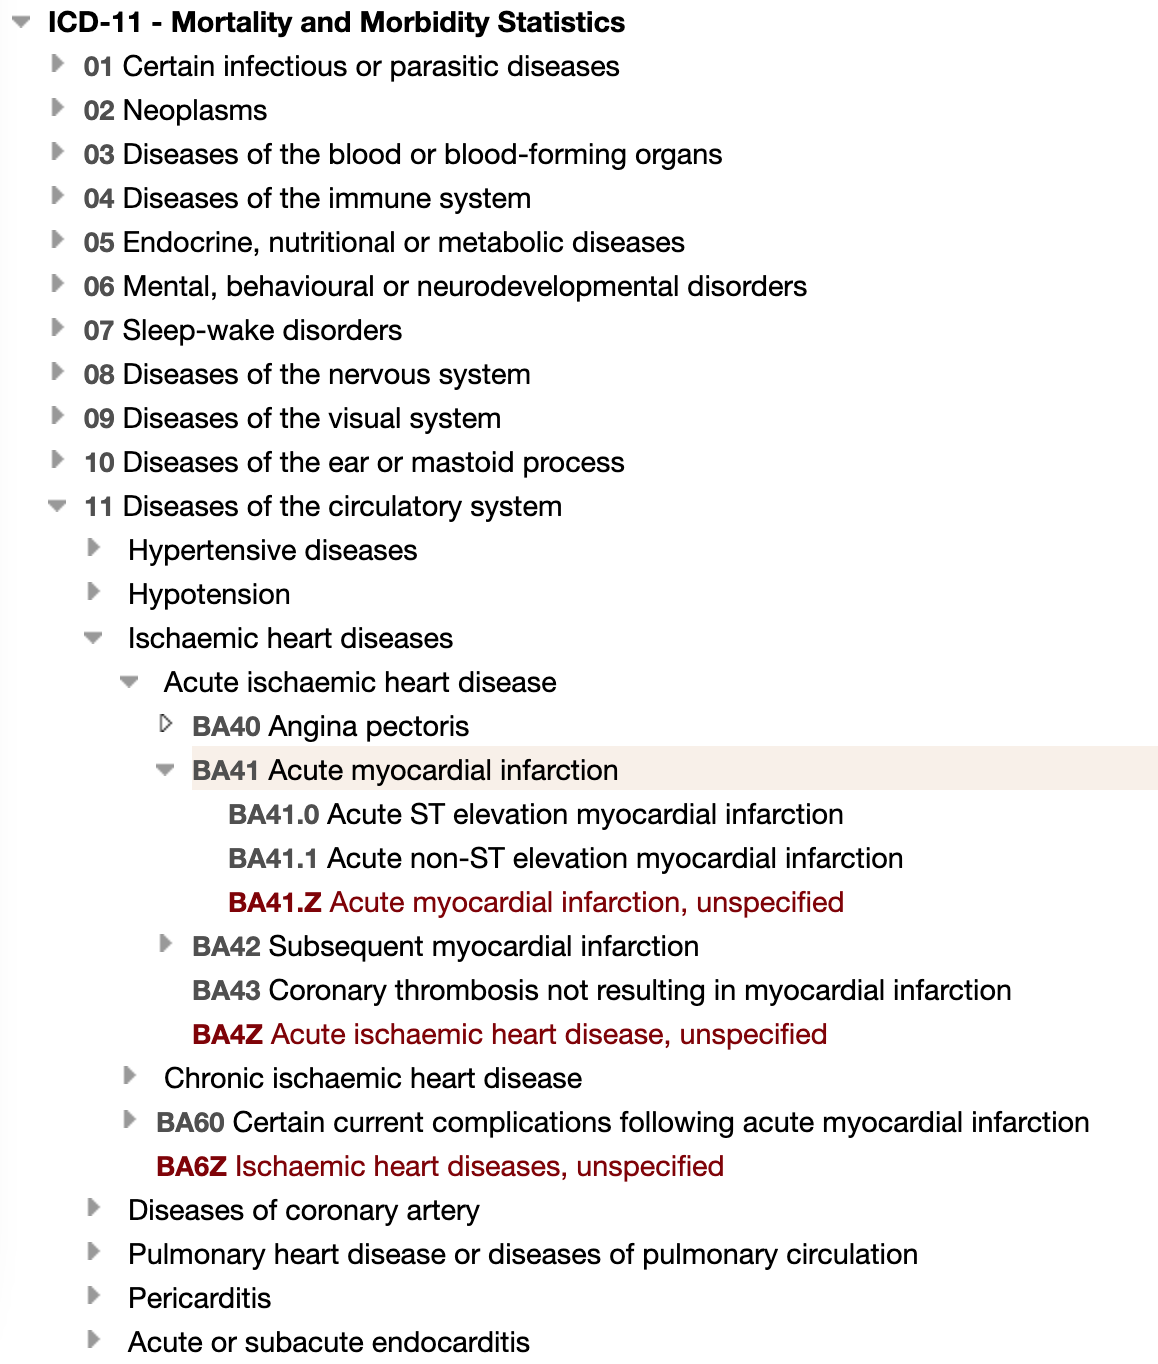
\includegraphics[width=0.8\textwidth]{icu_icd_mi}
    \caption{ICD Codes}
    \vspace{12px}
    The International Classification of Diseases (ICD) is a taxonomy of all medical conditions maintained by the World Health Organization.  "Acute myocardial infarction", for example, is a descendant of "Acute ischemic heart diseases", which itself is a descendant of "Ischemic heart diseases", which itself is a descendant of "Diseases of the circulatory system".  "Acute myocardial infarction" is then further subdivided if more granularity is required.
    \label{fig:icu_icd_mi}
    \end{figure}
}

\def \figIcuExampleWaveforms {
    \begin{figure}
    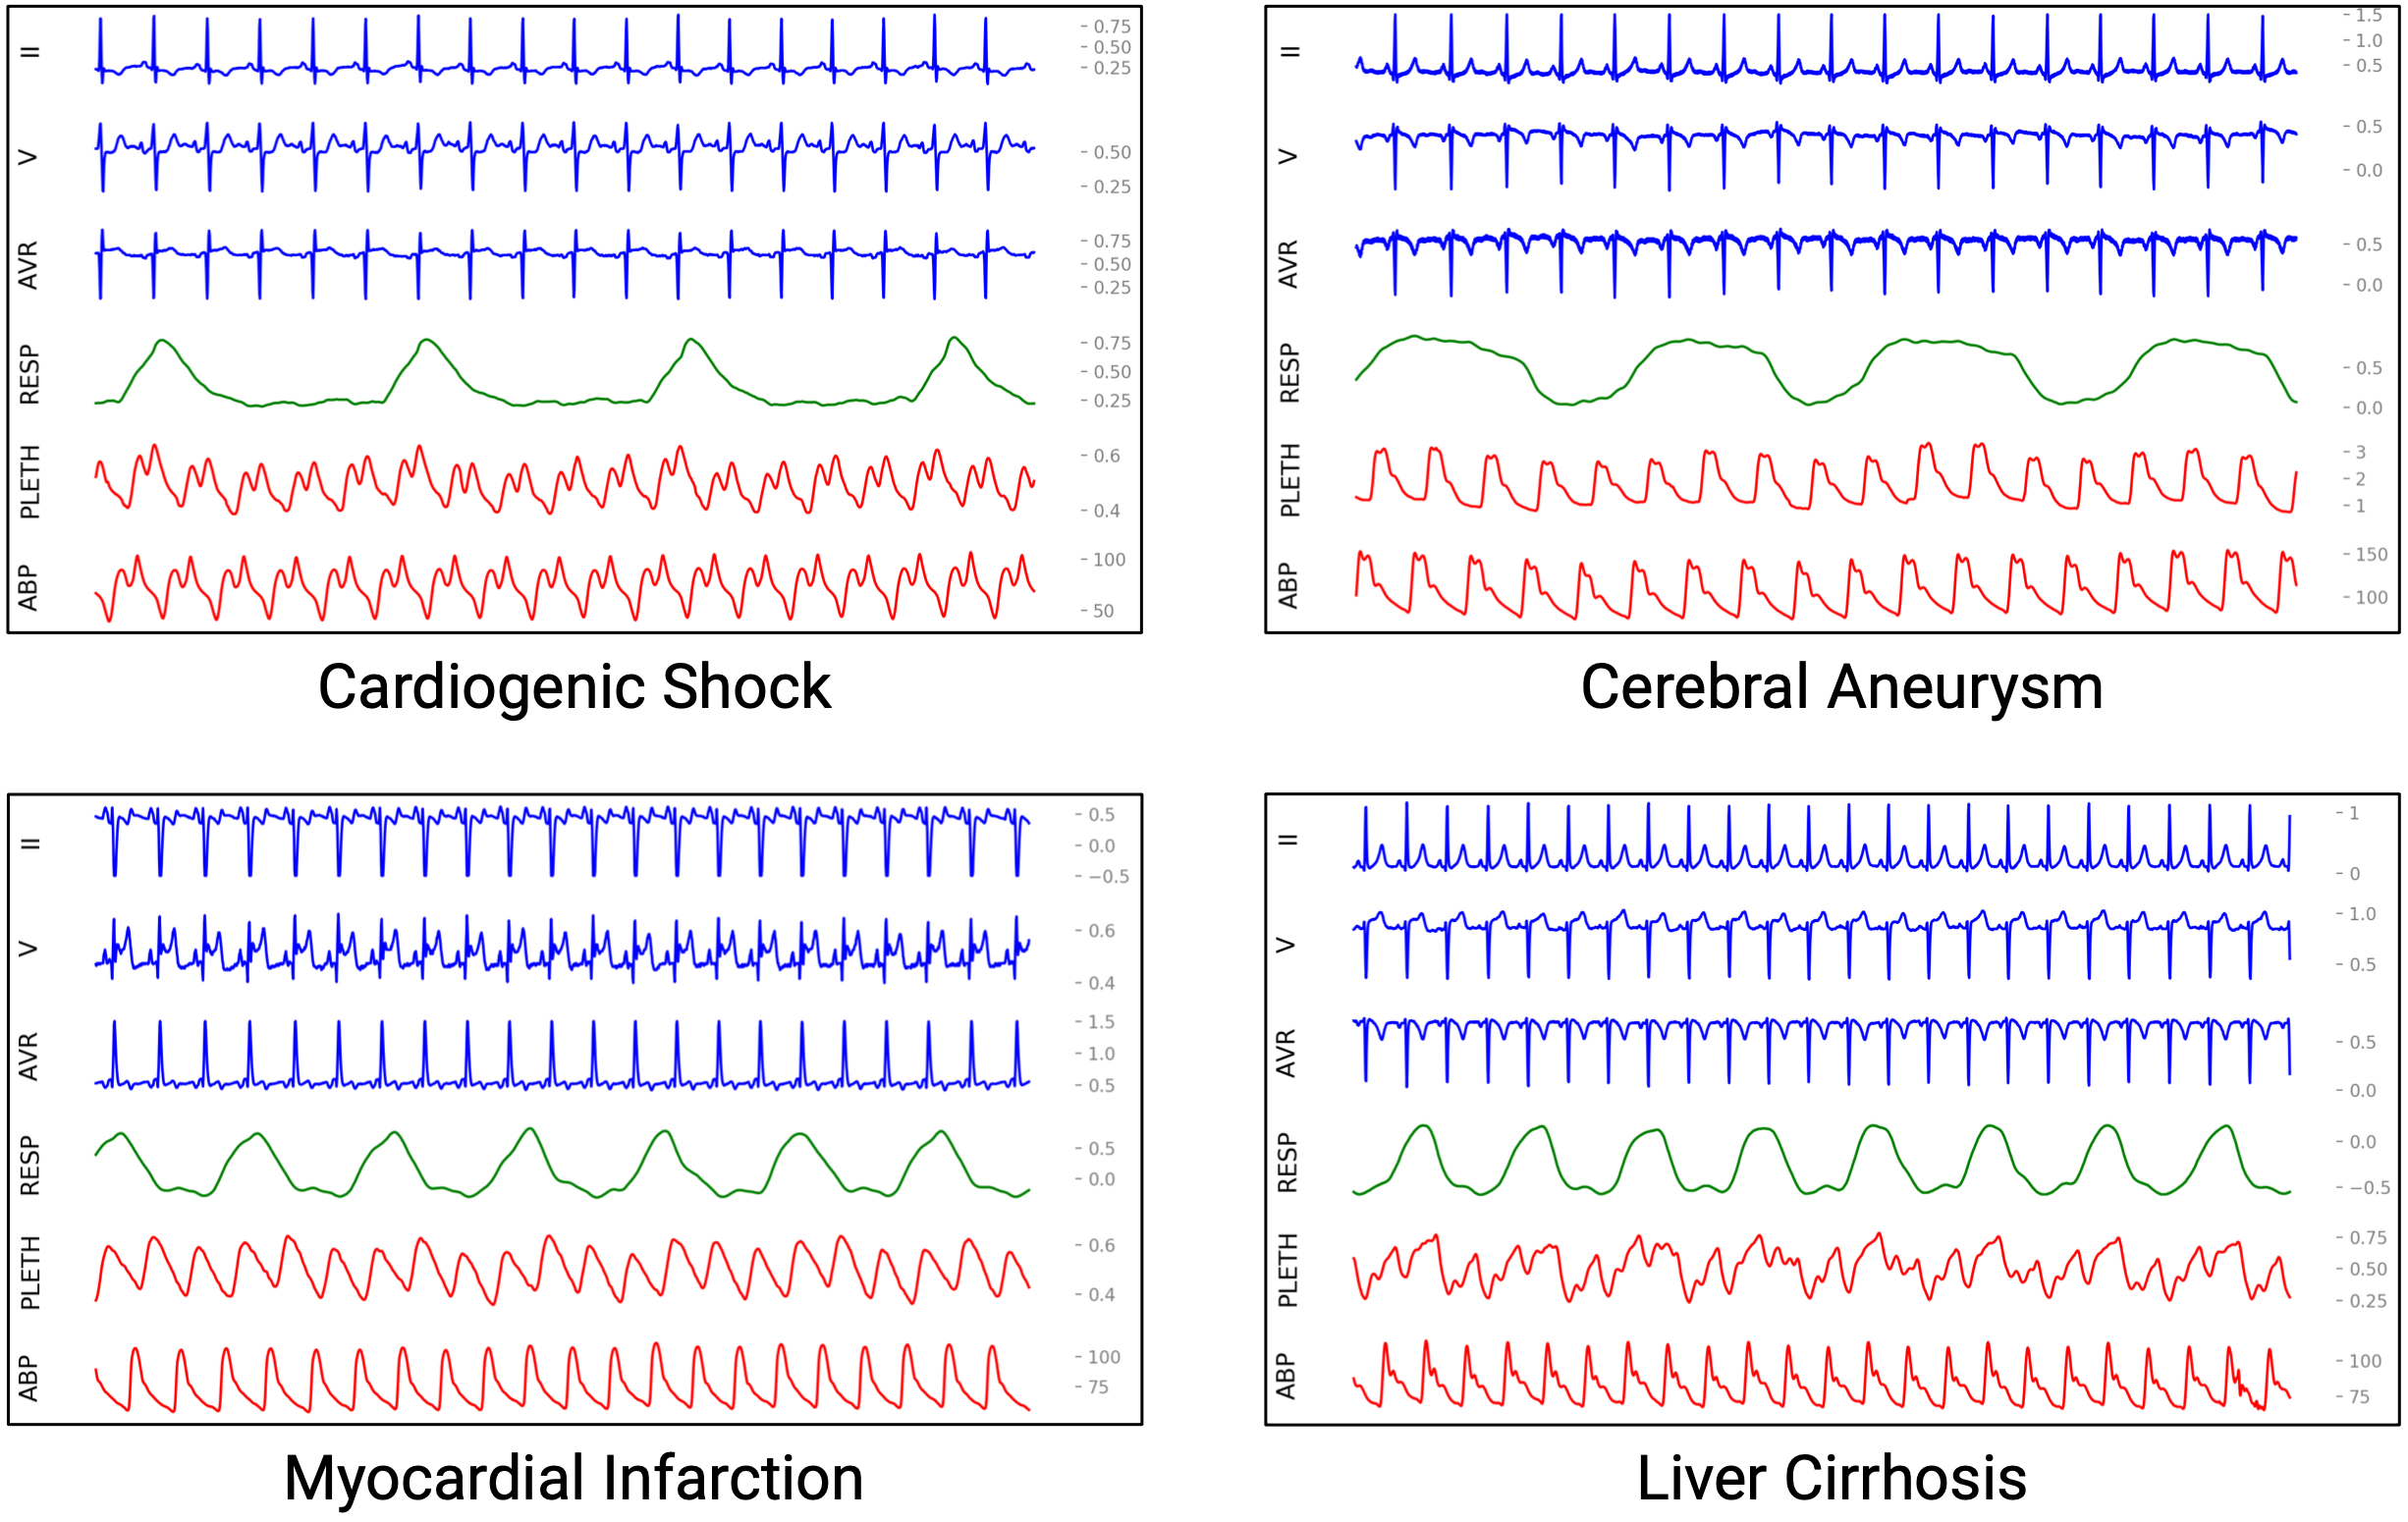
\includegraphics[width=\textwidth]{icu_example_inputs}
    \caption{Example inputs}
    \vspace{12px}
    Waveforms are sampled at 125Hz with 8 bit resolution.  An example contains 2048 samples, or about 16 seconds.  Waveform types include 3 ECG leads (II, V, AVR) shown in blue, respiration shown in in green, and photoplethysmogram and arterial blood pressure, both shown in red.  An example is labeled with a set of ICD codes.  For simplicity, examples here are shown that were correctly detected as having a given condition.  In the upper left we see an example that was correctly flagged for cardiogenic shock.  The the upper right we have an example of a detected cerebral aneurysm.  In the lower left and right we have examples of myocardial infarction and liver cirrhosis.
    \label{fig:icu_example_waveforms}
    \end{figure}
}

\def \figIcuModelArch {
    \begin{figure}
    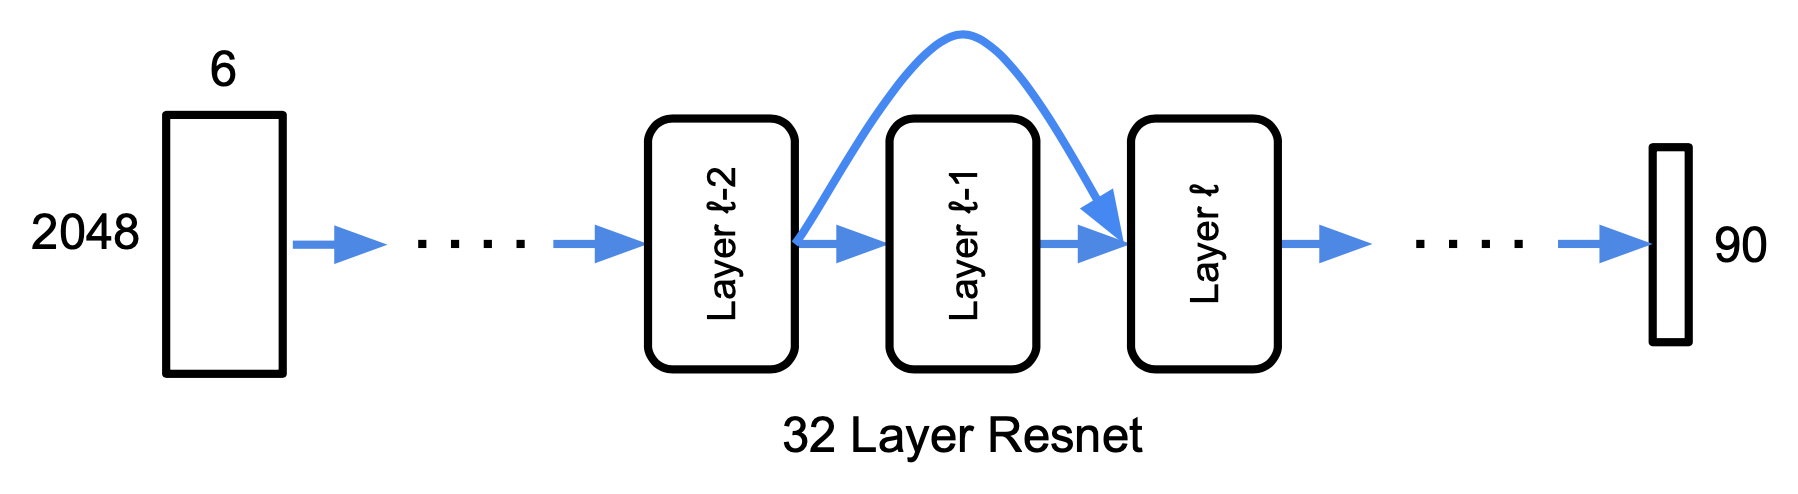
\includegraphics[width=\textwidth]{icu_model_arch}
    \caption{Model architecture}
    \vspace{12px}
    A 32 layer 1D ConvNet with residual layers was trained on inputs of $k$ by 2048.  During training time, $k = 15$, and during inference time $k = 6$.  The discrepancy in $k$ is due to the fact that not all waveforms are present for every patient.  The patients in the validation and test sets are restricted to those who have all 6 of the required waveforms measured.  During training, missing waveforms are input as 0 vectors.  The net outputs 90 probabilities, 1 for each of the 90 ICD codes trained on.  Each example can have multiple diagnoses associated with it.  The loss is the mean of all 90 binary cross entropies.
    \label{fig:icu_model_arch}
    \end{figure}
}

\def \figIcuCardioProb {
    \begin{figure}
    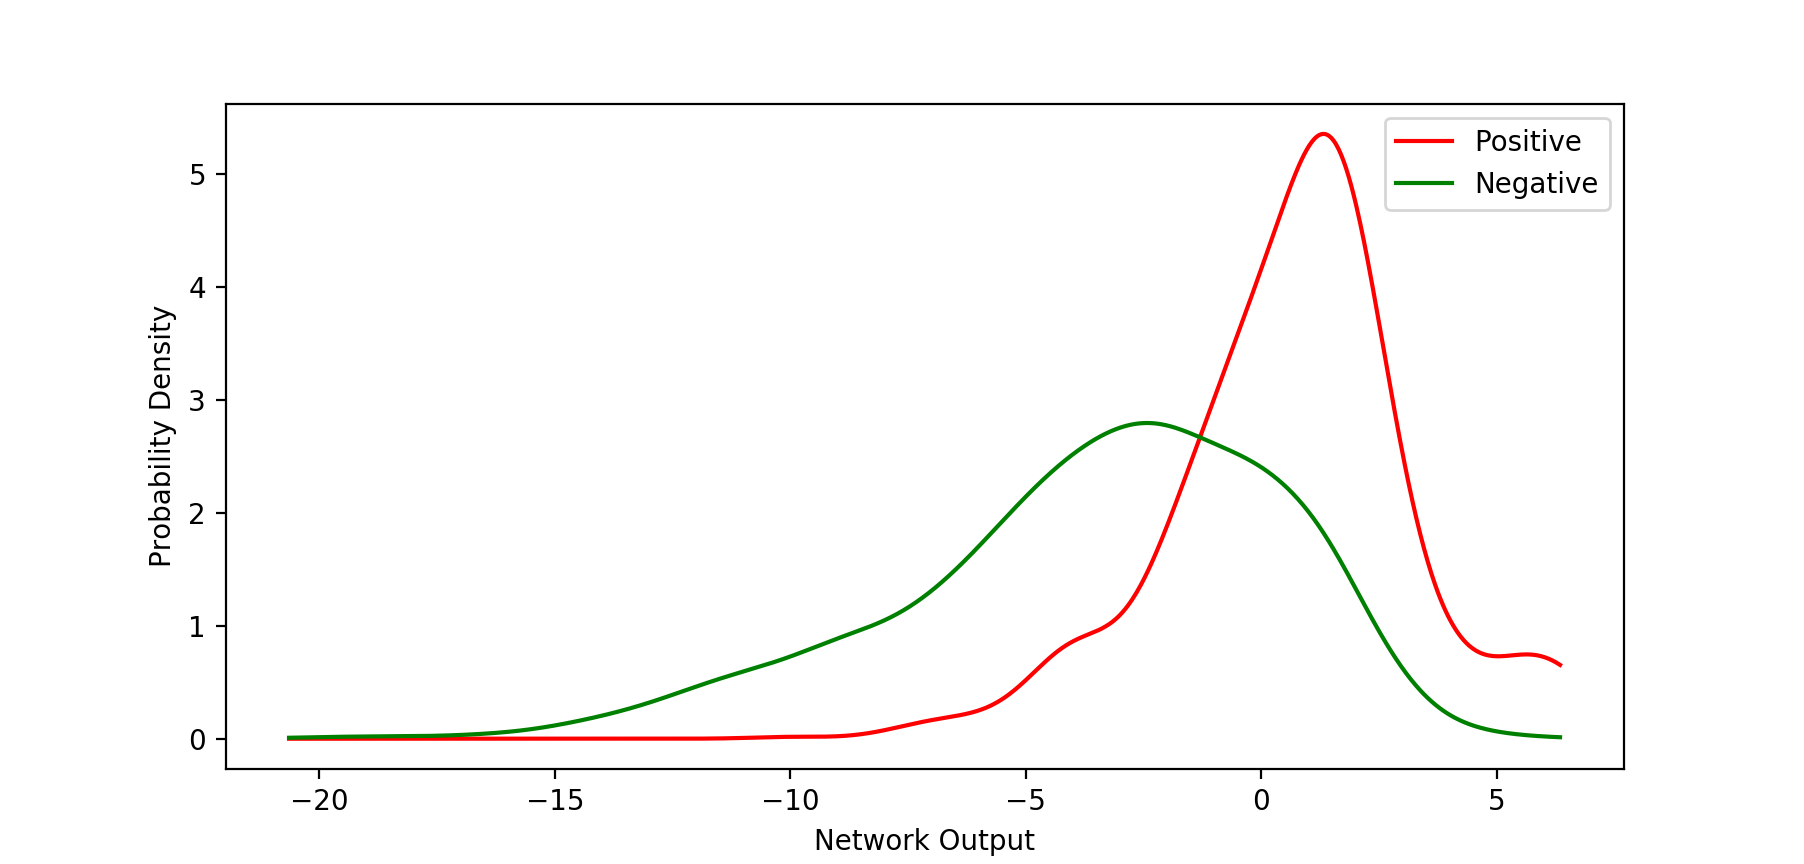
\includegraphics[width=\textwidth]{icu_cardio_prob}
    \caption{Cardiogenic Shock Separation}
    \vspace{12px}
    Conditional distributions of network output given the diagnosis is positive or negative for cardiogenic shock.
    \label{fig:icu_cardio_prob}
    \end{figure}
}

\def \figIcuCardioSens {
    \begin{figure}
    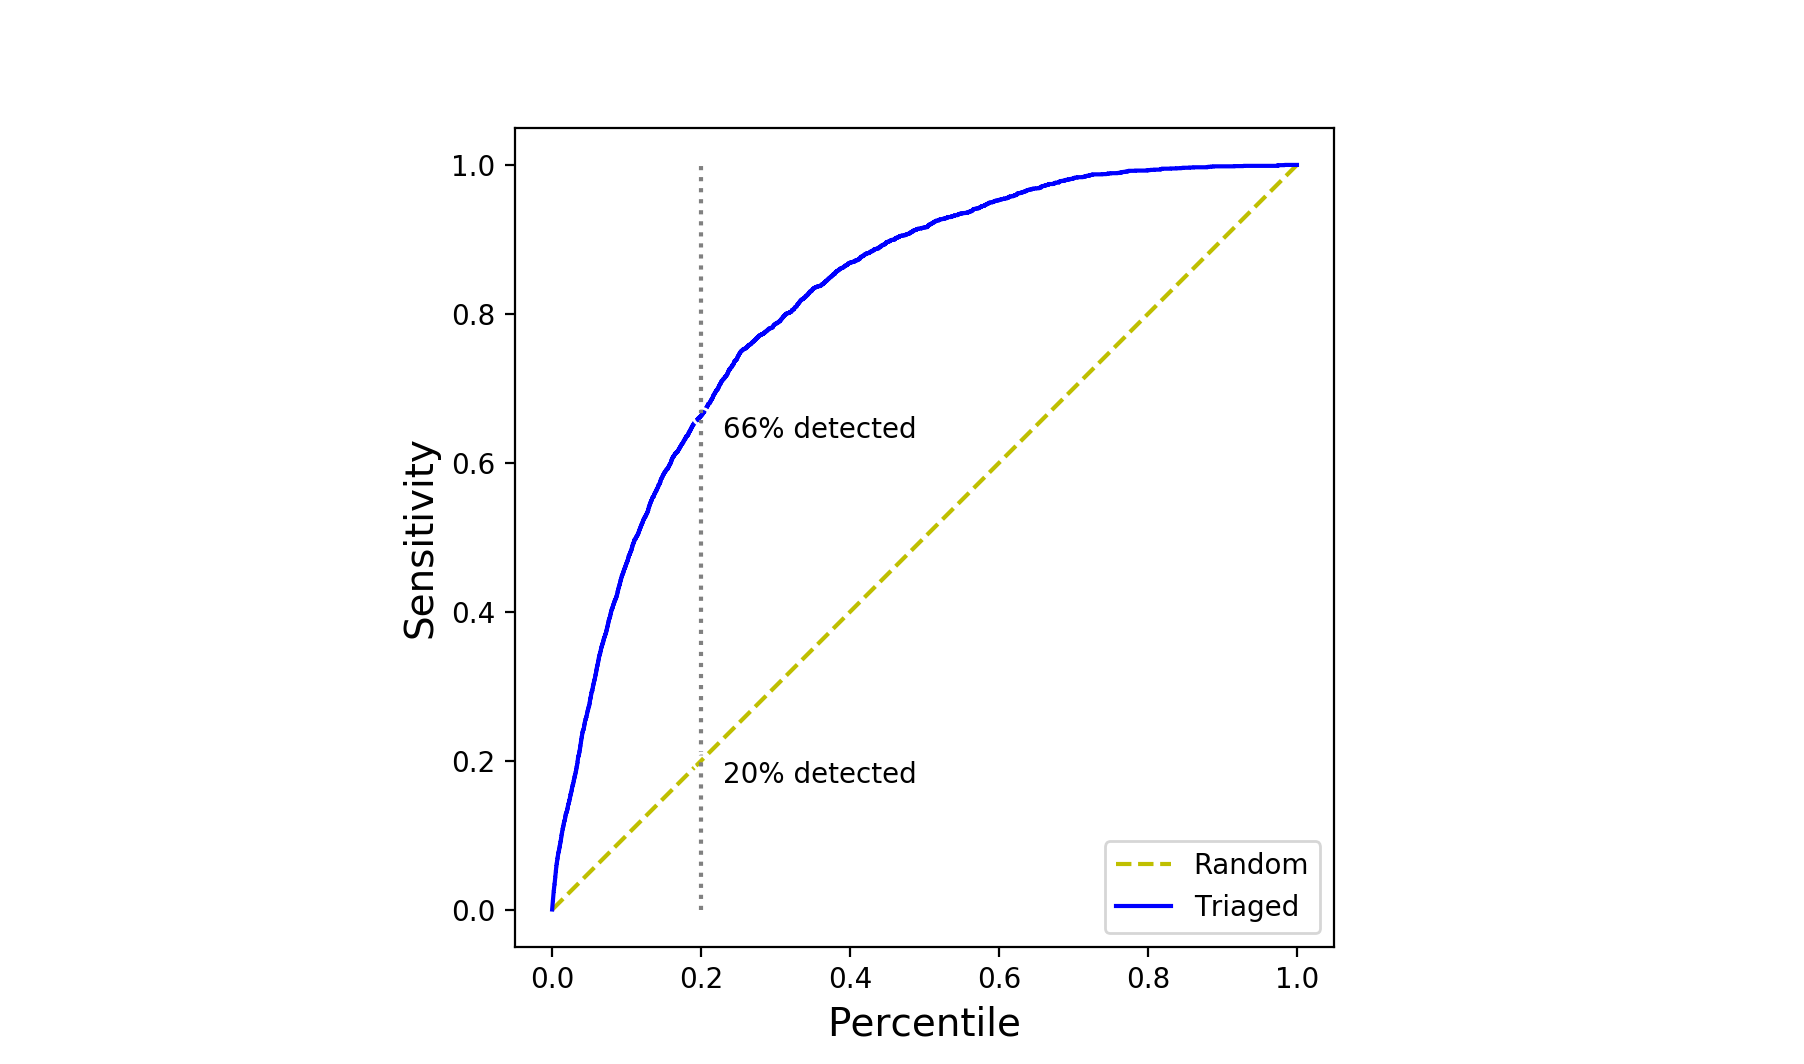
\includegraphics[width=\textwidth]{icu_cardio_sens}
    \caption{Cardiogenic Shock Effective Sensitivity}
    \vspace{12px}
    Effective sensitivity of the network for detecting a cardiogenic shock.  As an example, assume only 20\% of the patients can be tested with an expensive but perfect test. Using the net to flag the 20 percentile patients at highest risk for further testing would detect 66\% of the cases.
    \label{fig:icu_cardio_sens}
    \end{figure}
}

\def \figIcuSystolicProb {
    \begin{figure}
    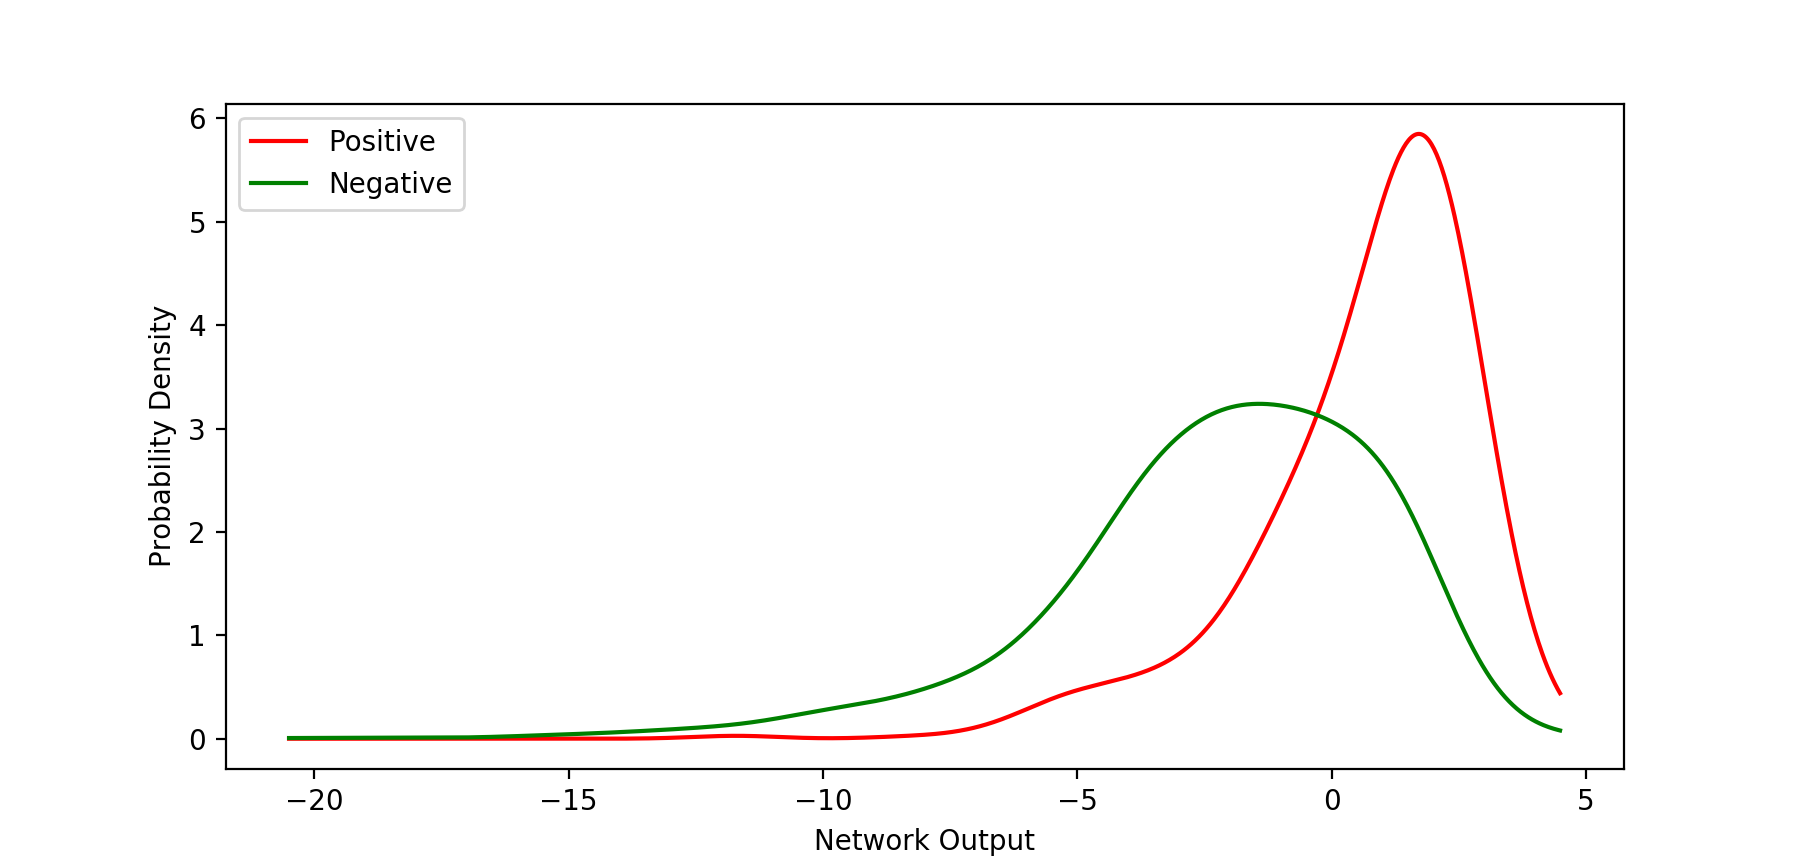
\includegraphics[width=\textwidth]{icu_systolic_prob}
    \caption{Systolic Heart Failure Separation}
    \vspace{12px}
    Conditional distributions of network output given the diagnosis is positive or negative for systolic heart failure.
    \label{fig:icu_systolic_prob}
    \end{figure}
}

\def \figIcuSystolicSens {
    \begin{figure}
    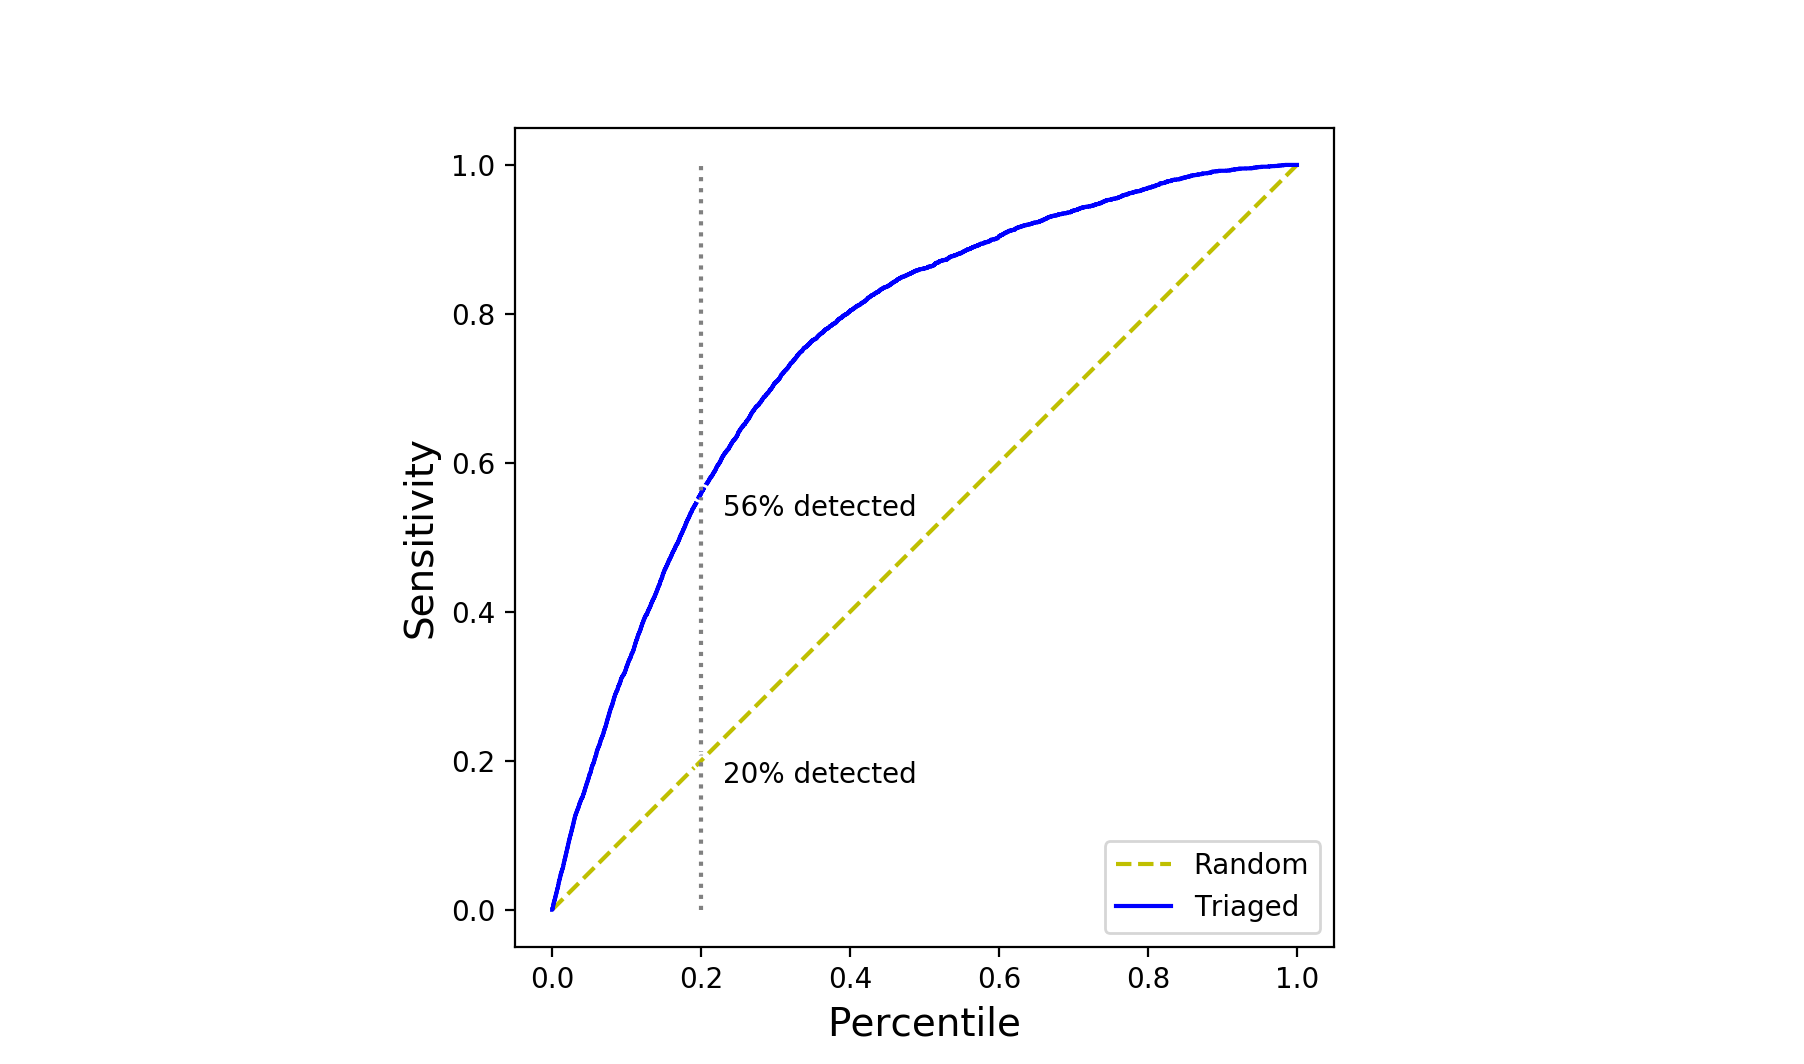
\includegraphics[width=\textwidth]{icu_systolic_sens}
    \caption{Systolic Heart Failure Effective Sensitivity}
    \vspace{12px}
    Effective sensitivity of the network for detecting systolic heart failure.  As an example, assume only 20\% of the patients can be tested with an expensive but perfect test. Using the net to flag the 20 percentile patients at highest risk for further testing would detect 56\% of the cases.
    \label{fig:icu_systolic_sens}
    \end{figure}
}

\def \figIcuCerebralProb {
    \begin{figure}
    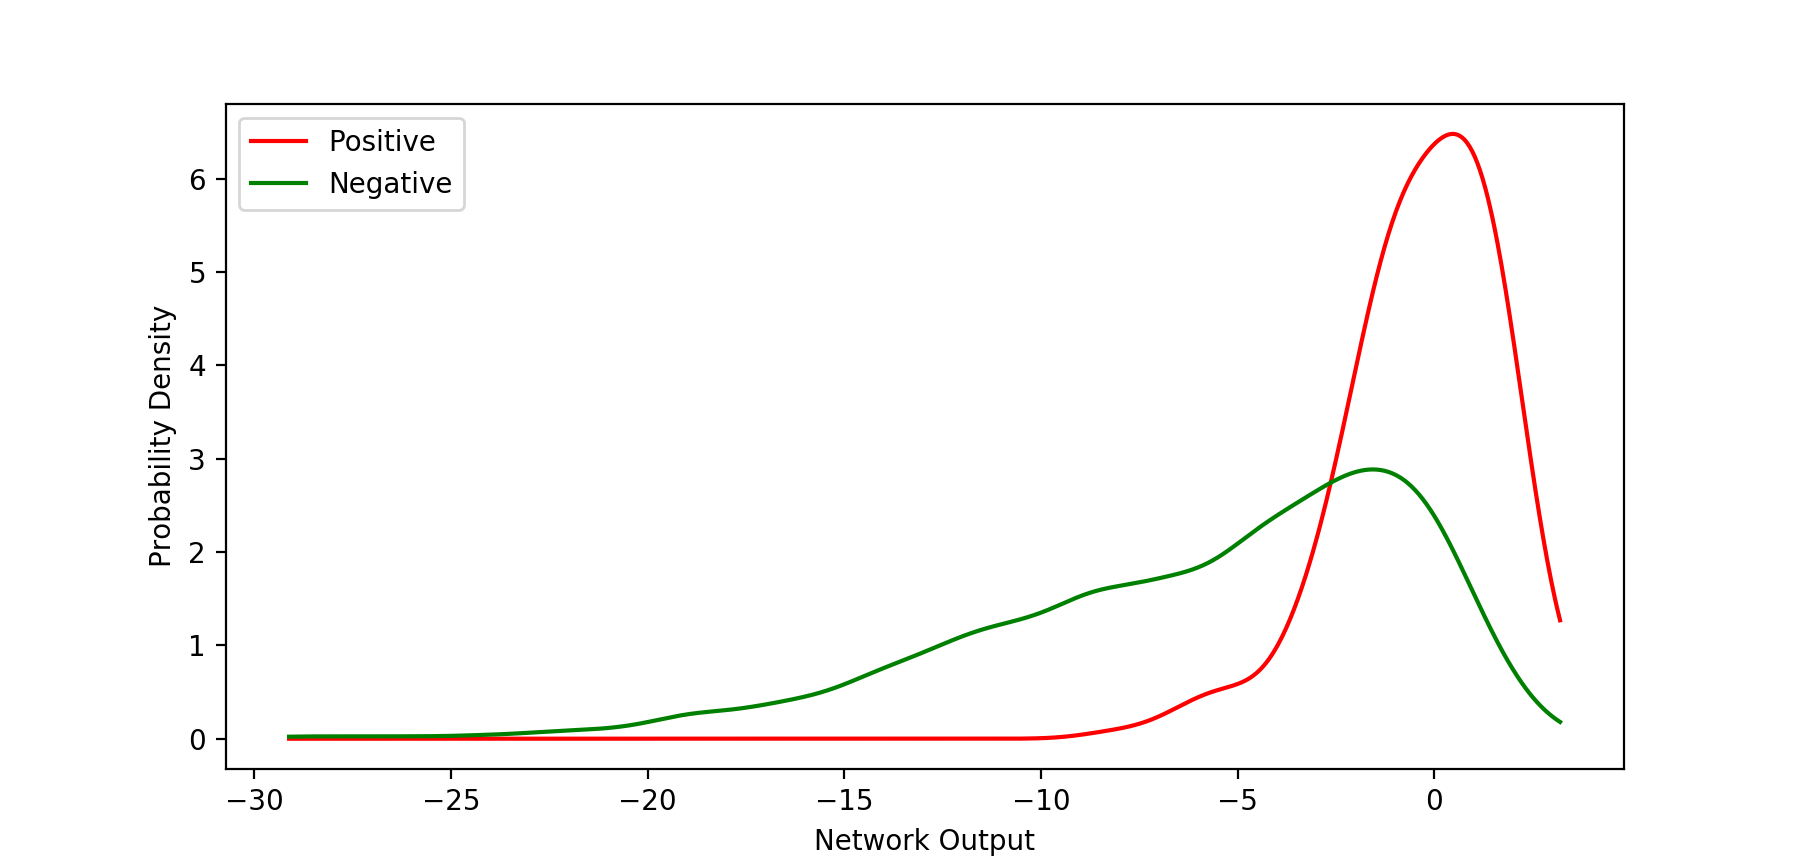
\includegraphics[width=\textwidth]{icu_cerebral_prob}
    \caption{Cerebral Aneurysm Separation}
    \vspace{12px}
    Conditional distributions of network output given the diagnosis is positive or negative for cerebral aneurysm.
    \label{fig:icu_cerebral_prob}
    \end{figure}
}

\def \figIcuCerbralSens {
    \begin{figure}
    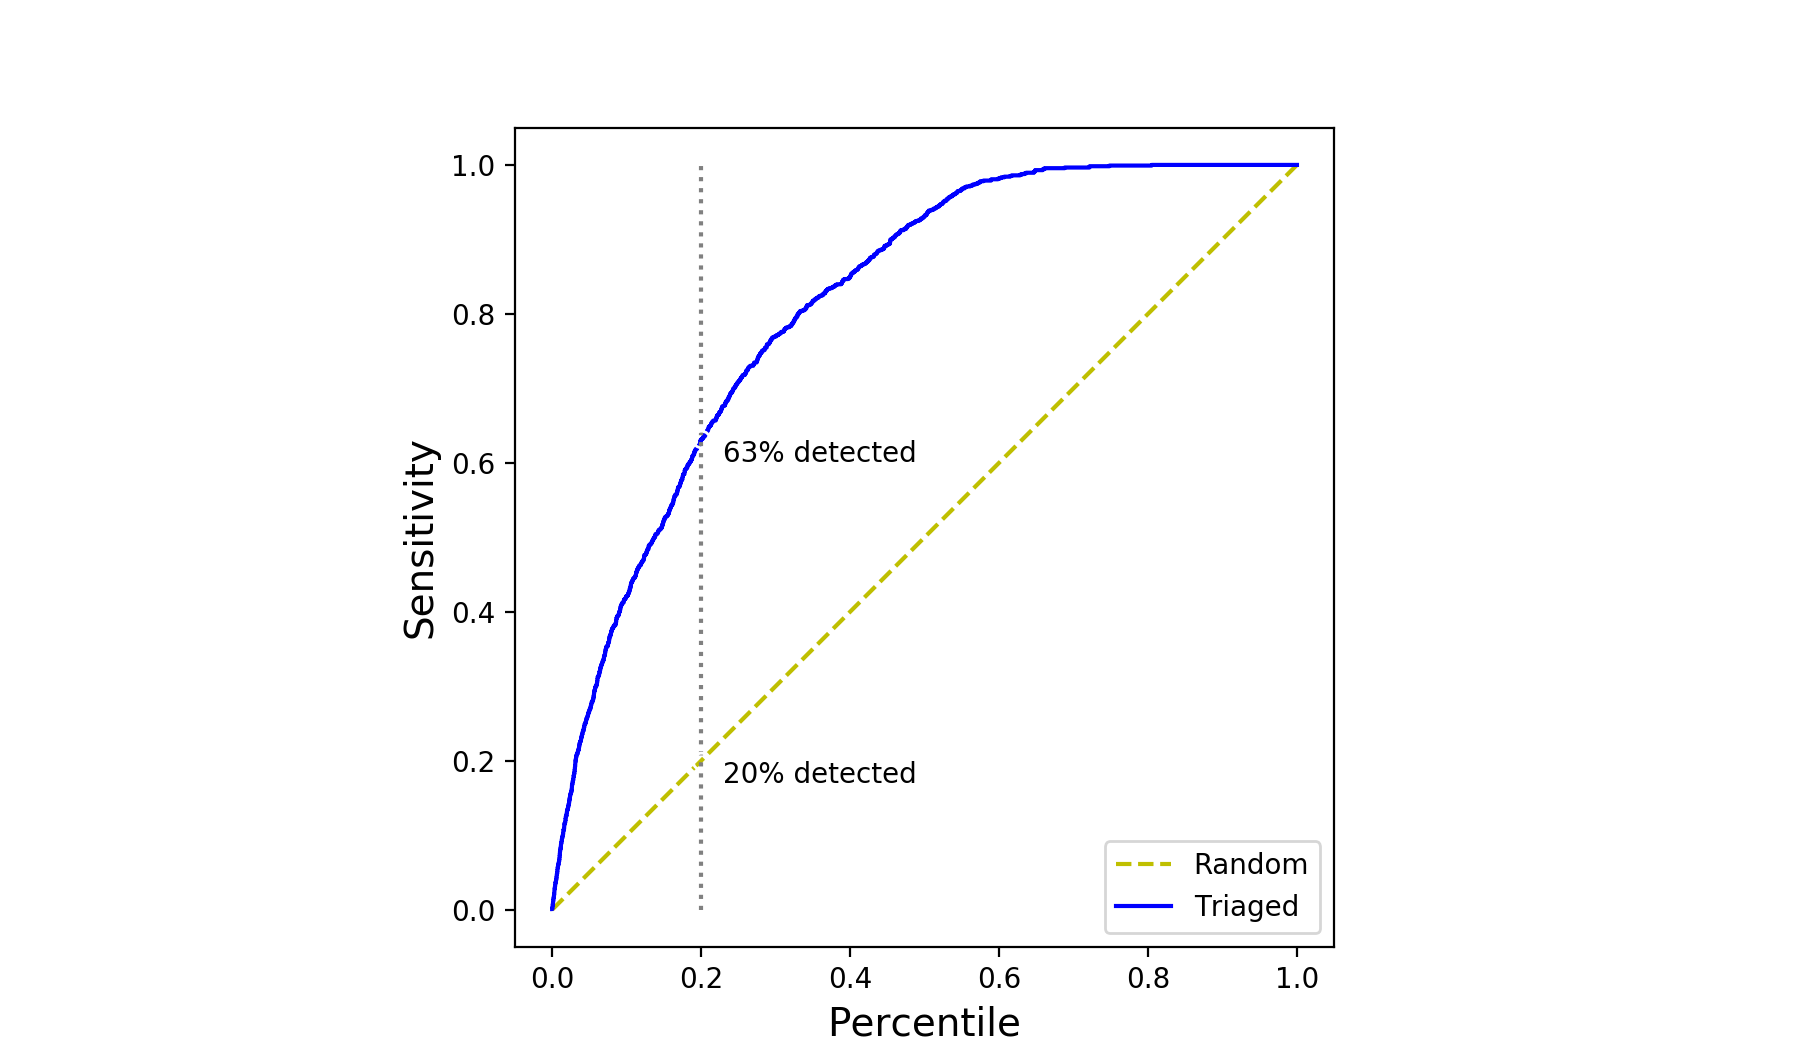
\includegraphics[width=\textwidth]{icu_cerebral_sens}
    \caption{Cerebral Aneurysm Effective Sensitivity}
    \vspace{12px}
    Effective sensitivity of the network for detecting a cerebral aneurysm.  As an example, assume only 20\% of the patients can be tested with an expensive but perfect test. Using the net to flag the 20 percentile patients at highest risk for further testing would detect 63\% of the cases.
    \label{fig:icu_cerebral_sens}
    \end{figure}
}

\def \figIcuMyocardProb {
    \begin{figure}
    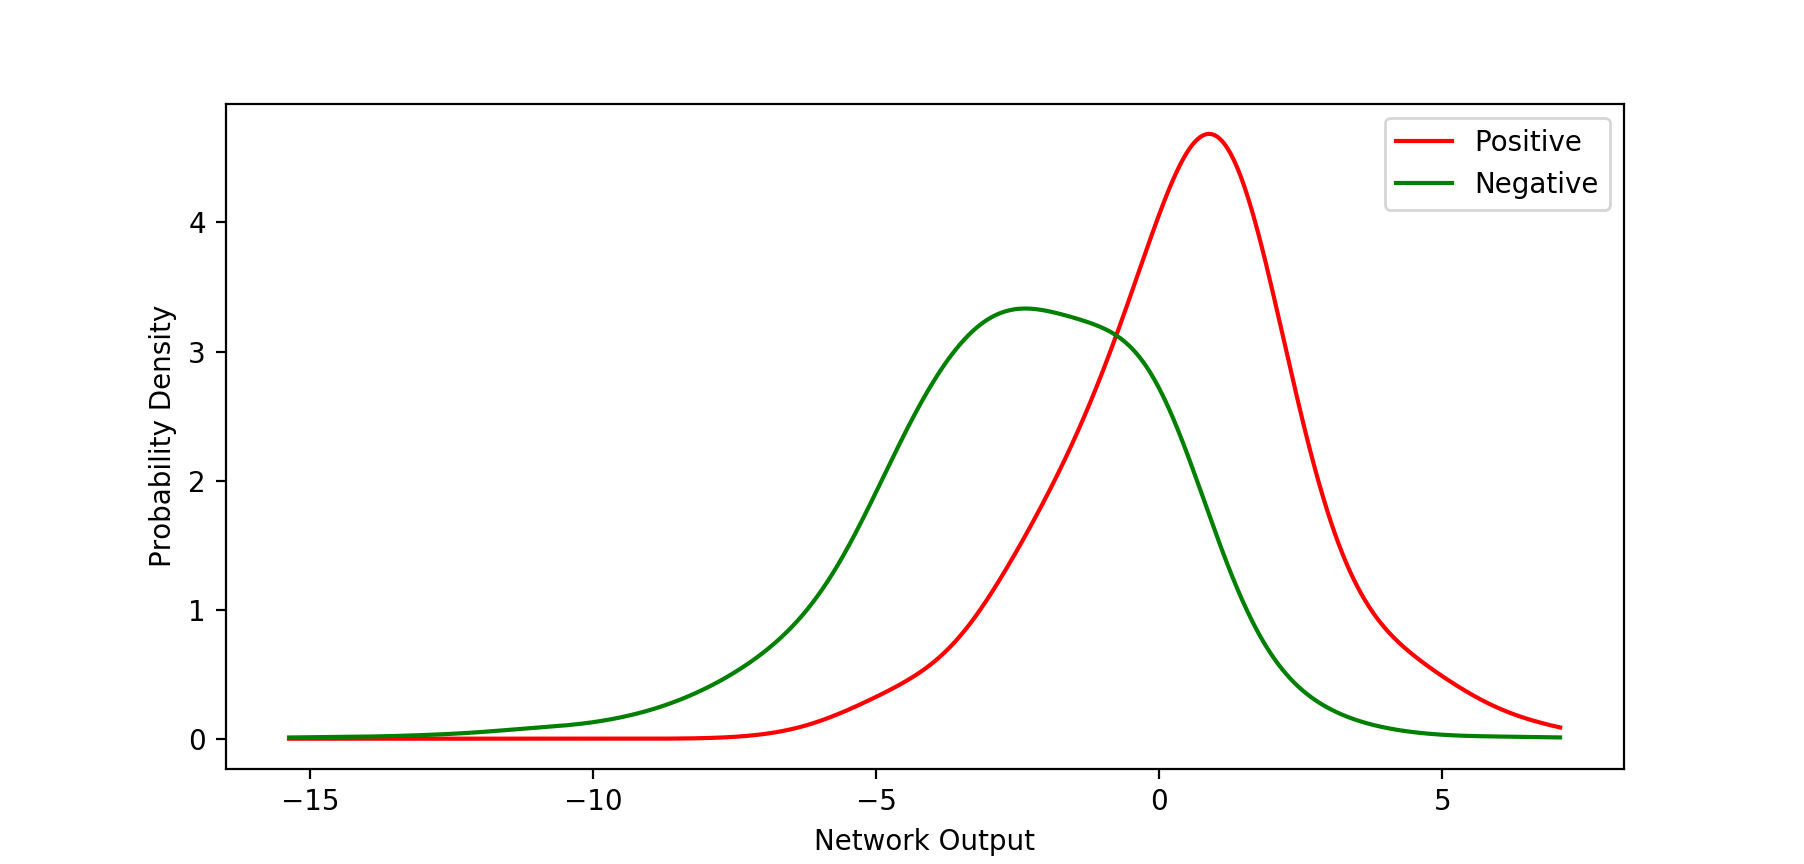
\includegraphics[width=\textwidth]{icu_myocard_prob}
    \caption{Myocardial Infarction Separation}
    \vspace{12px}
    Conditional distributions of network output given the diagnosis is positive or negative for myocardial infarction.
    \label{fig:icu_myocard_prob}
    \end{figure}
}

\def \figIcuMyocardSens {
    \begin{figure}
    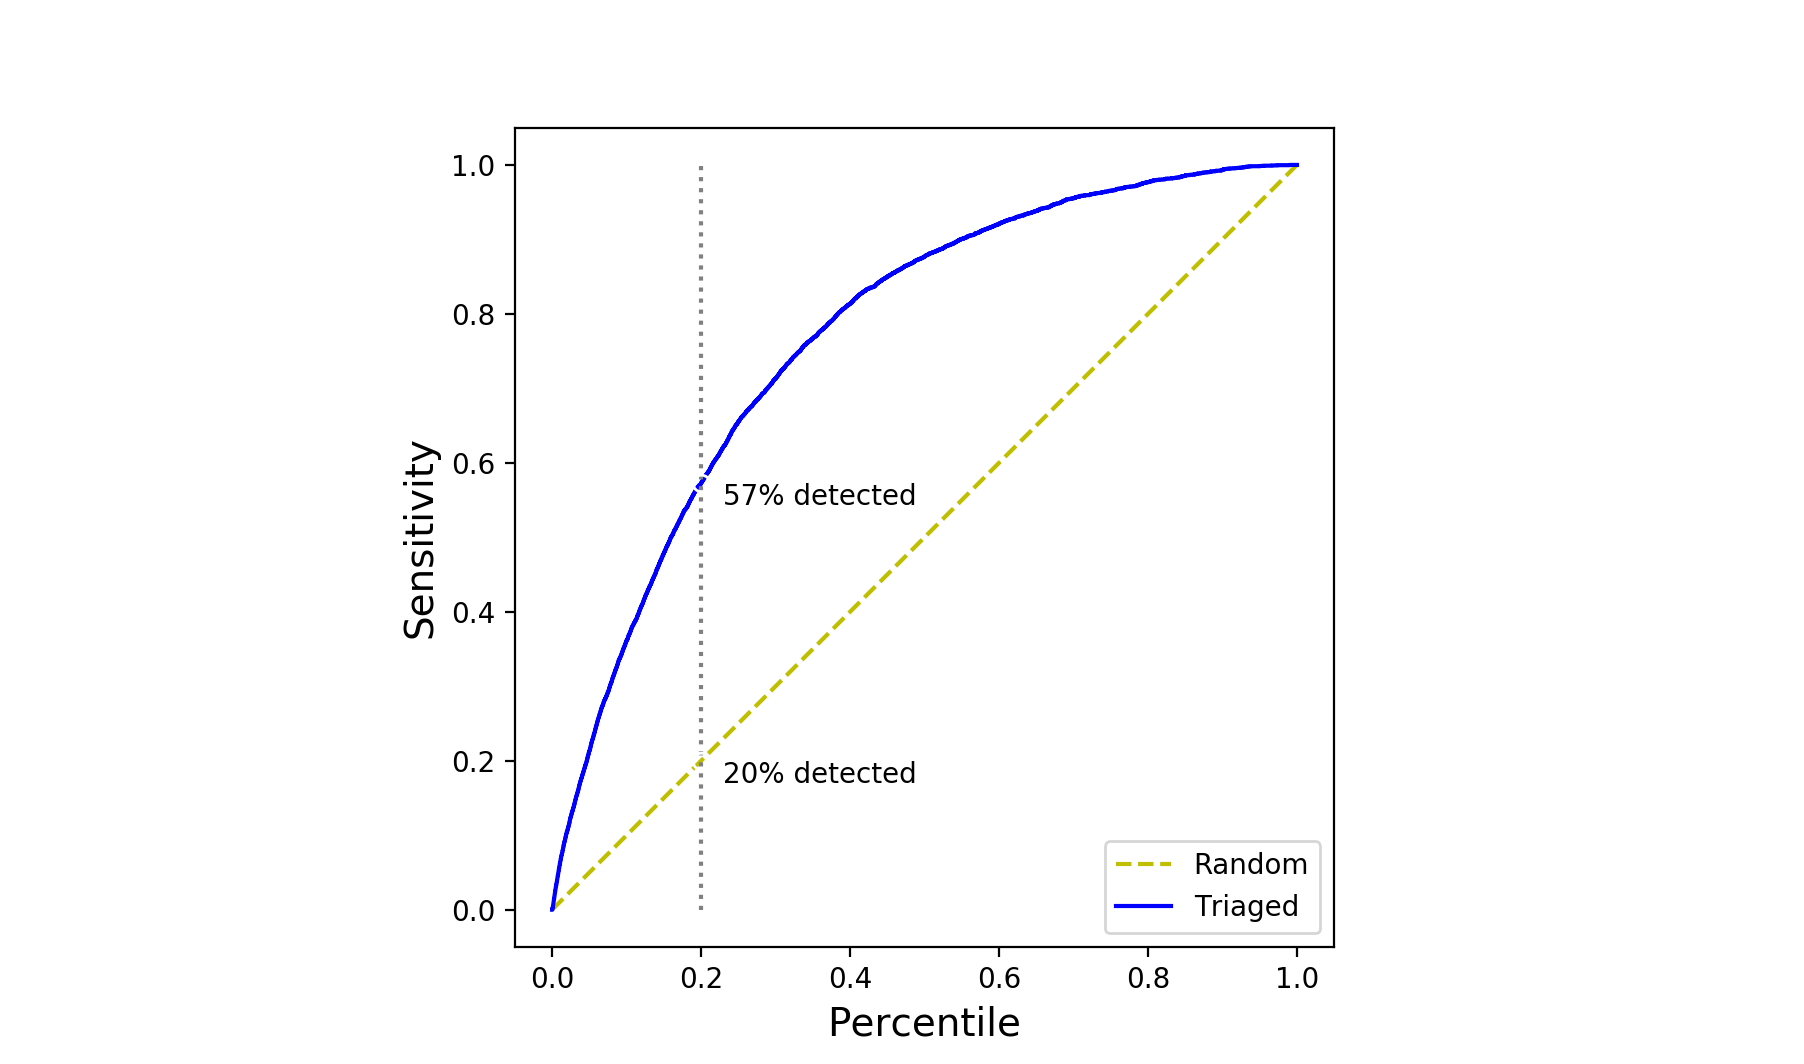
\includegraphics[width=\textwidth]{icu_myocard_sens}
    \caption{Myocardial Infarction Effective Sensitivity}
    \vspace{12px}
    Effective sensitivity of the network for detecting a myocardial infarction.  As an example, assume only 20\% of the patients can be tested with an expensive but perfect test. Using the net to flag the 20 percentile patients at highest risk for further testing would detect 57\% of the cases.
    \label{fig:icu_myocard_sens}
    \end{figure}
}

\def \figIcuRelativeRisk {
    \begin{figure}
    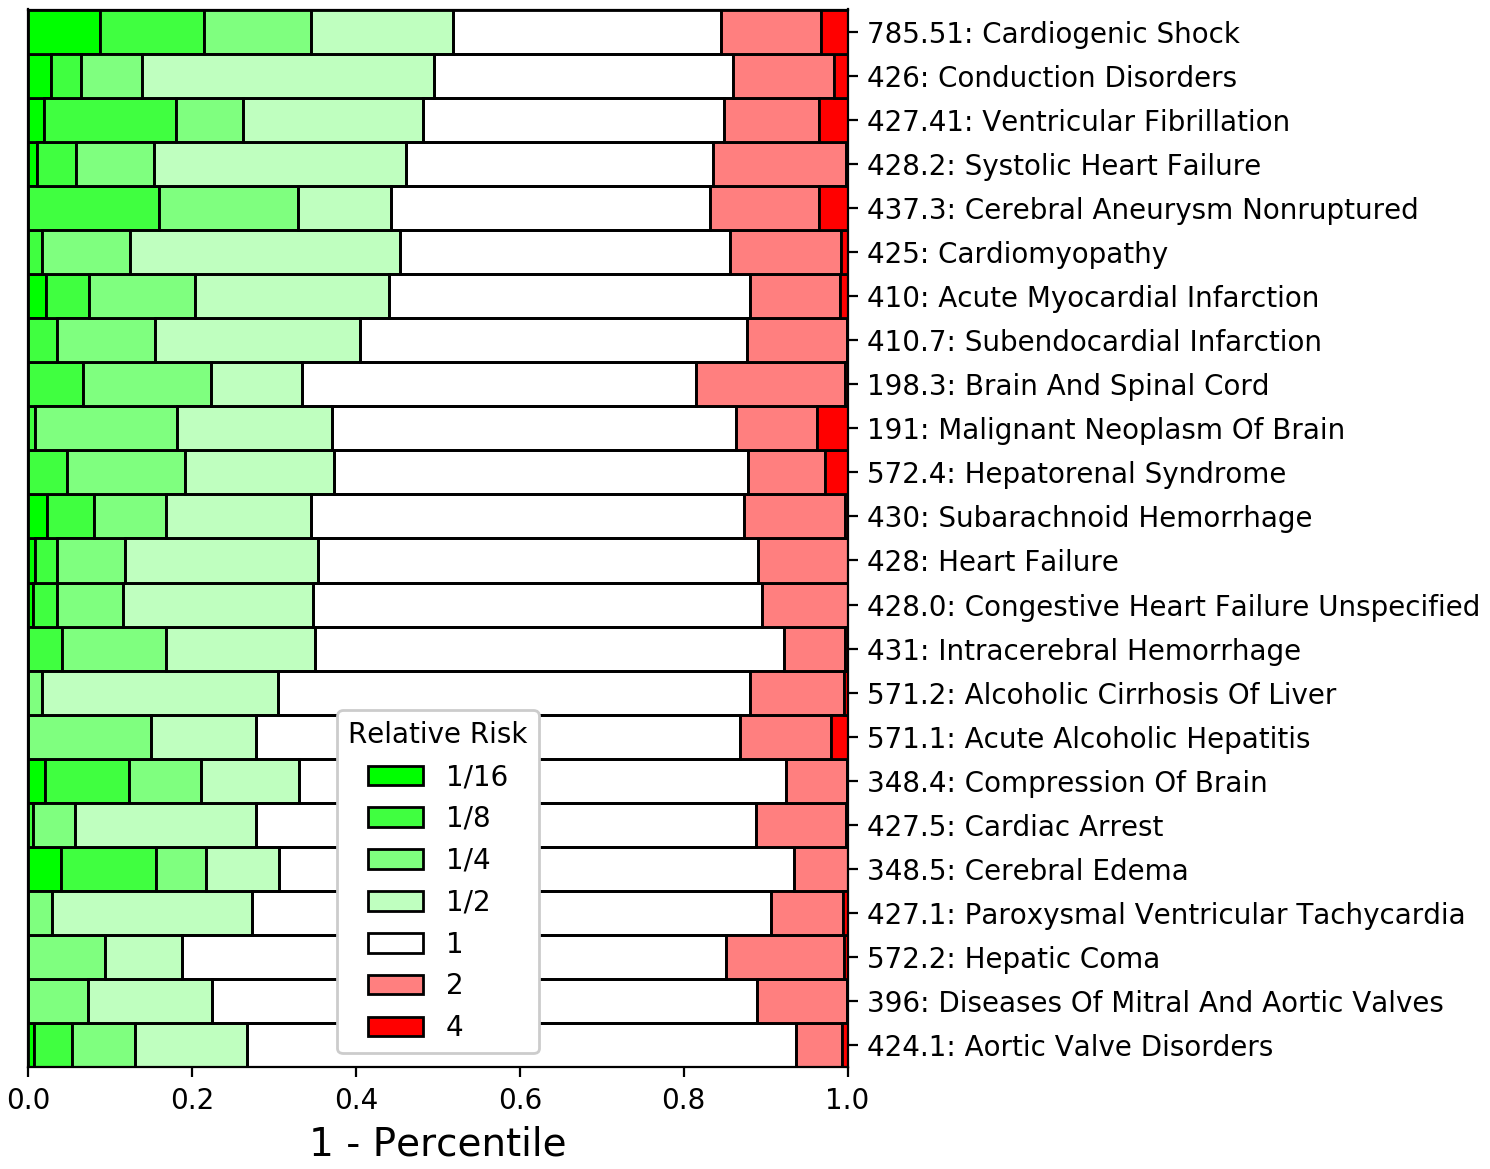
\includegraphics[width=\textwidth]{icu_relative_risk}
    \caption{Relative risk}
    \vspace{12px}
    Patients are placed into estimated risk categories of powers of 2.  For example, a patient in the 1/4 risk category of systolic heart failure is estimated to be between 1/4 and 1/8 as likely to be diagnosed with systolic heart failure.  For cardiogenic shock, about half of the patients can be placed into a low risk category.
    \label{fig:icu_relative_risk}
    \end{figure}
}

\def \figIcuActualRisk {
    \begin{figure}
    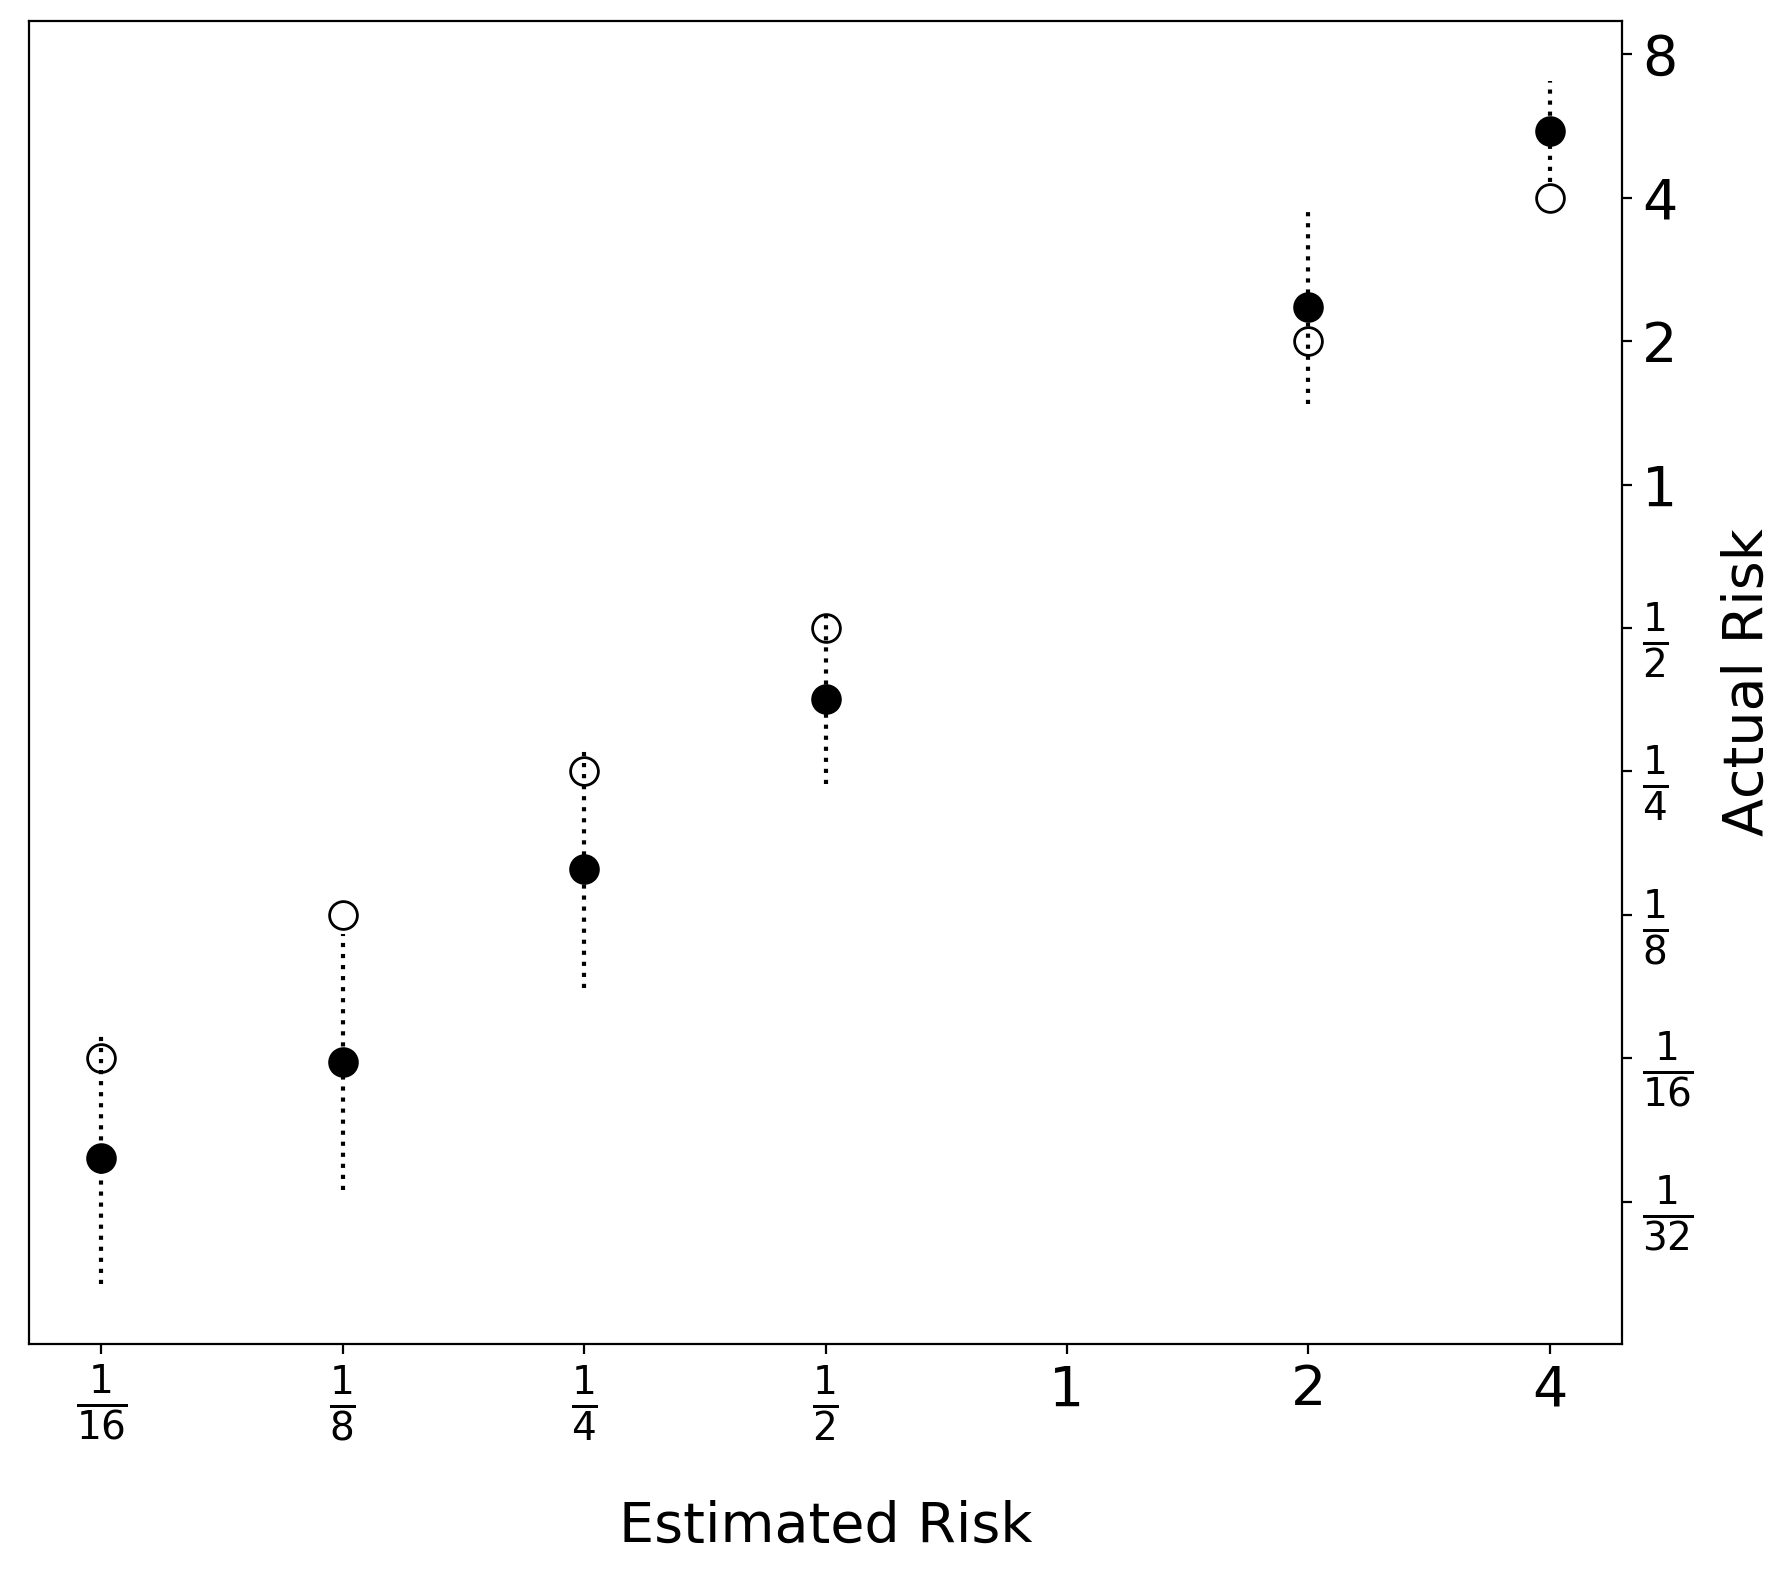
\includegraphics[width=\textwidth]{icu_actual_risk}
    \caption{Actual risk}
    \vspace{12px}
    Risk categories are valid.  For each risk category an actual risk can be computed with error bars.  The error bars represent the fact that there are 90 conditions being predicted.  Ideally the low risk categories should have an actual risk lower than the estimated risk and the high risk categories should have a risk higher than the estimated risk.  This is due to the fact that risk categories represent an estimated risk $r$ in the range $2^n < r < 2^{n+1}$ for $n > 0$ (high risk) and $2^n > r > 2^{n+1}$ for $n < 0$ (low risk).  This indeed occurs as shown.
    \label{fig:icu_actual_risk}
    \end{figure}
}

\def \figIcuEmbeddingMethod {
    \begin{figure}
    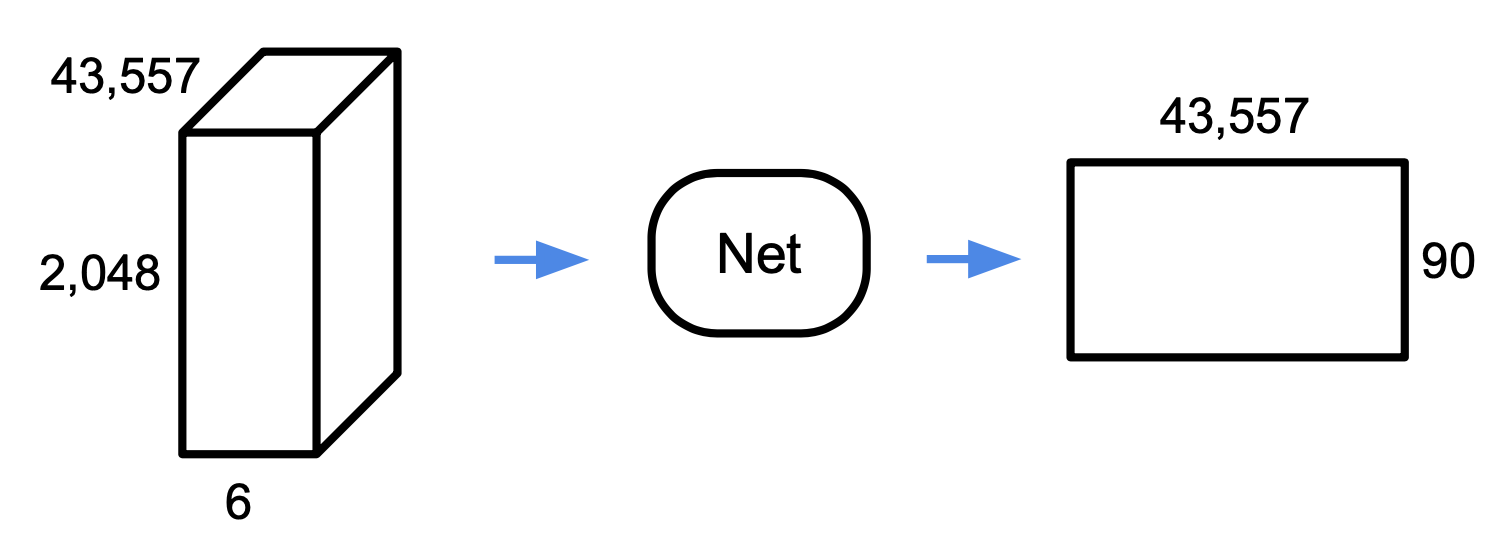
\includegraphics[width=\textwidth]{icu_embedding_method}
    \caption{ICD Embedding Method}
    \vspace{12px}
    To compute an embedding of ICD codes from what the net has learned, 43,557 examples are forward passed through the net producing a 43,557 by 90 matrix.  The 90 rows of this matrix represent 43,557 dimensional embeddings of the ICD codes.
    \label{fig:icu_embedding_method}
    \end{figure}
}

\def \figIcuIcdMap {
    \begin{figure}
    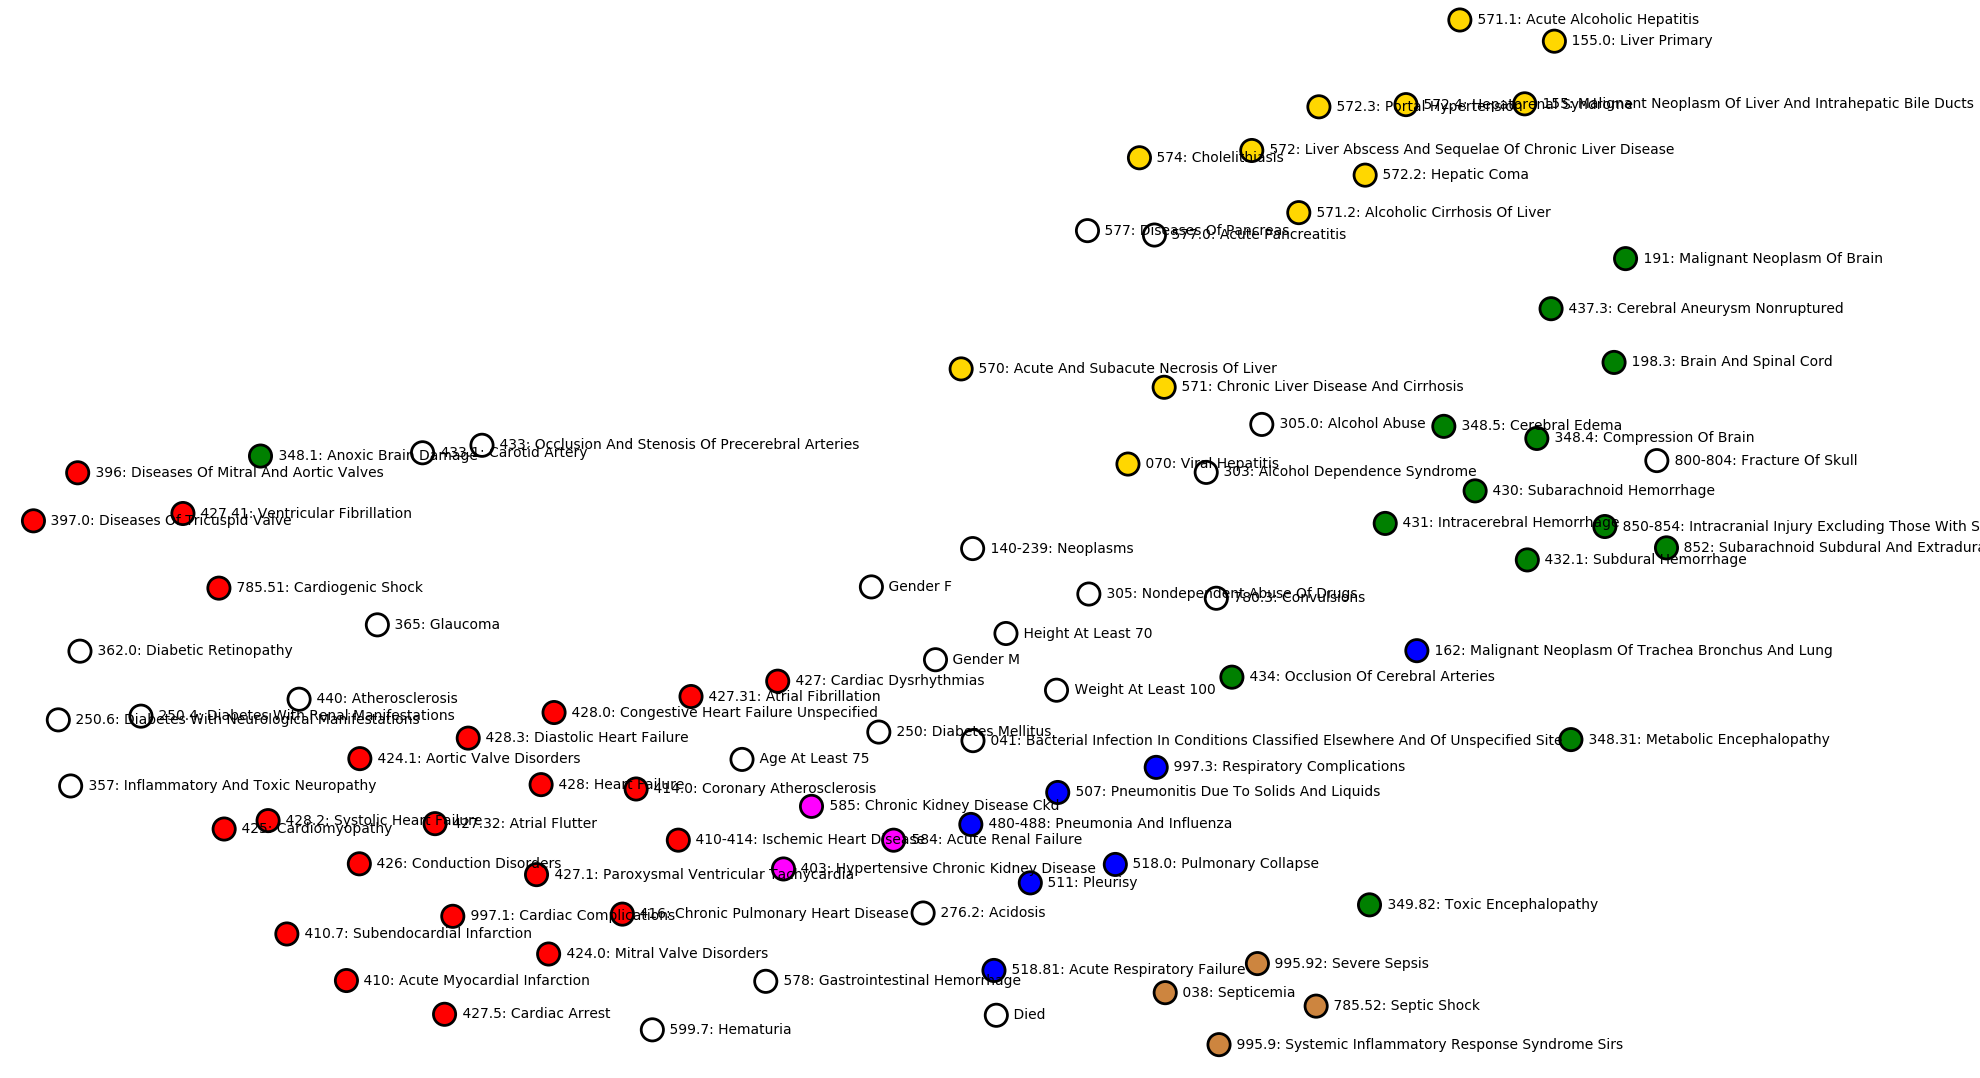
\includegraphics[width=\textwidth]{icu_icd_map}
    \caption{2D Projection of ICD Embedding}
    \vspace{12px}
    TSNE was applied to high dimensional ICD code embeddings to produce a 2D visualization of the ICD code space learned by the net.  Conditions affecting various organs are close together in this space.  Red circles are conditions that affect the heart.  These conditions include cardiogenic shock, coronary atherosclerosis, atrial flutter, systolic heart failure, and myocardial infarction.  Green circles are conditions that affect the brain.  These conditions include cerebral edema, brain cancer, cerebral aneurysm, intracerebral hemorrhage.  It is interesting that skull fracture found its way into this region.  Yellow circles are conditions that affect the liver.  These conditions include cirrhosis, hepatitis, and liver cancer.  It is interesting that alcohol abuse and alcohol dependence syndrome found their way into this region, and are also close to the brain conditions.  Blue circles are conditions that affect the lungs.  These conditions include pulmonary collapse, pneumonia, and acute respiratory failure.  This embedding also puts similar ICD codes together that may be far apart in the ICD taxonomy.  For example consider ICD code 785.52: Septic Shock, ICD code 995.92: Severe Sepsis, and ICD code 038: Septicemia.  The nearest common ancestor of these ICD codes in the taxonomy is the root of the entire taxonomy of all medical conditions that exist.  But the net learned that they were similar semantically based on the waveforms it was trained with.
    \label{fig:icu_icd_map}
    \end{figure}
}

\def \figIcuMaps {
    \begin{figure}
    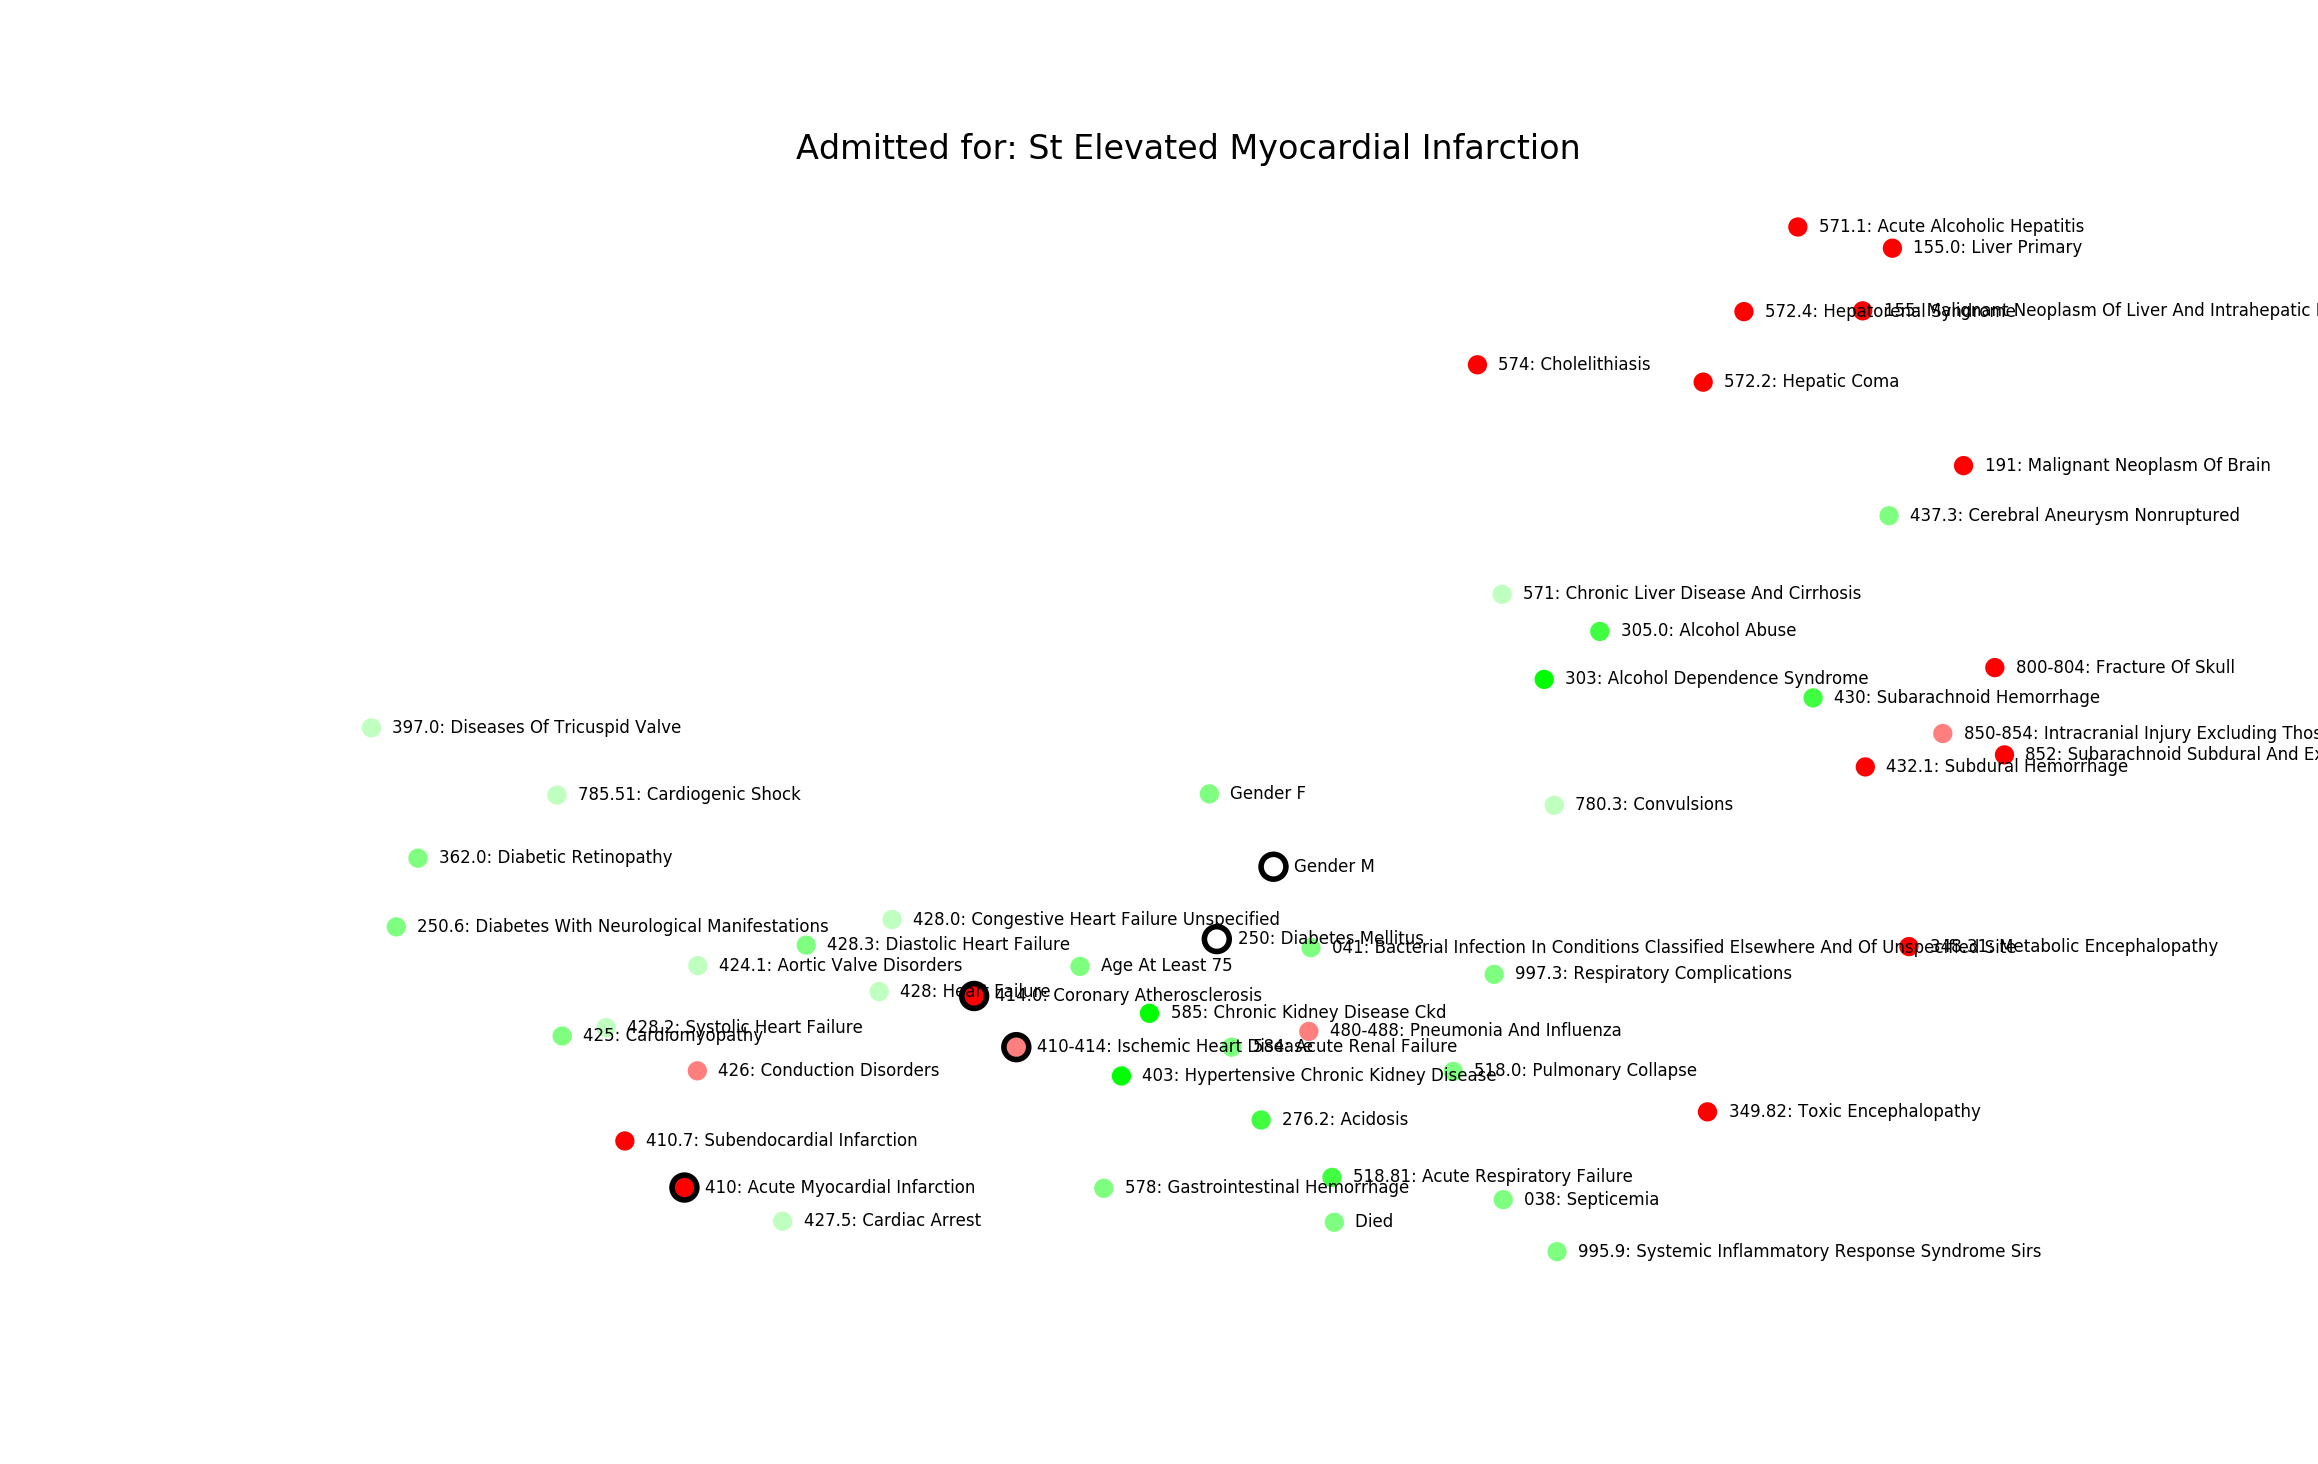
\includegraphics[width=\textwidth]{icu_map_mi}
    \caption{Semantic Inference Myocardial Infarction}
    \vspace{12px}
    This patient was admitted for "ST Elevated Myocardial Infarction".  The neural net correctly predicted that they had low risk of kidney conditions, death, and many heart conditions (colored green).  It predicted high risk of liver conditions and various heart conditions including myocardial infarction and coronary atherosclerosis (colored red).  The patients was eventually in fact diagnosed with myocardial infarction and coronary atherosclerosis among other things (circled in black).
    \label{fig:icu_map_mi}
    \end{figure}
    
    \begin{figure}
    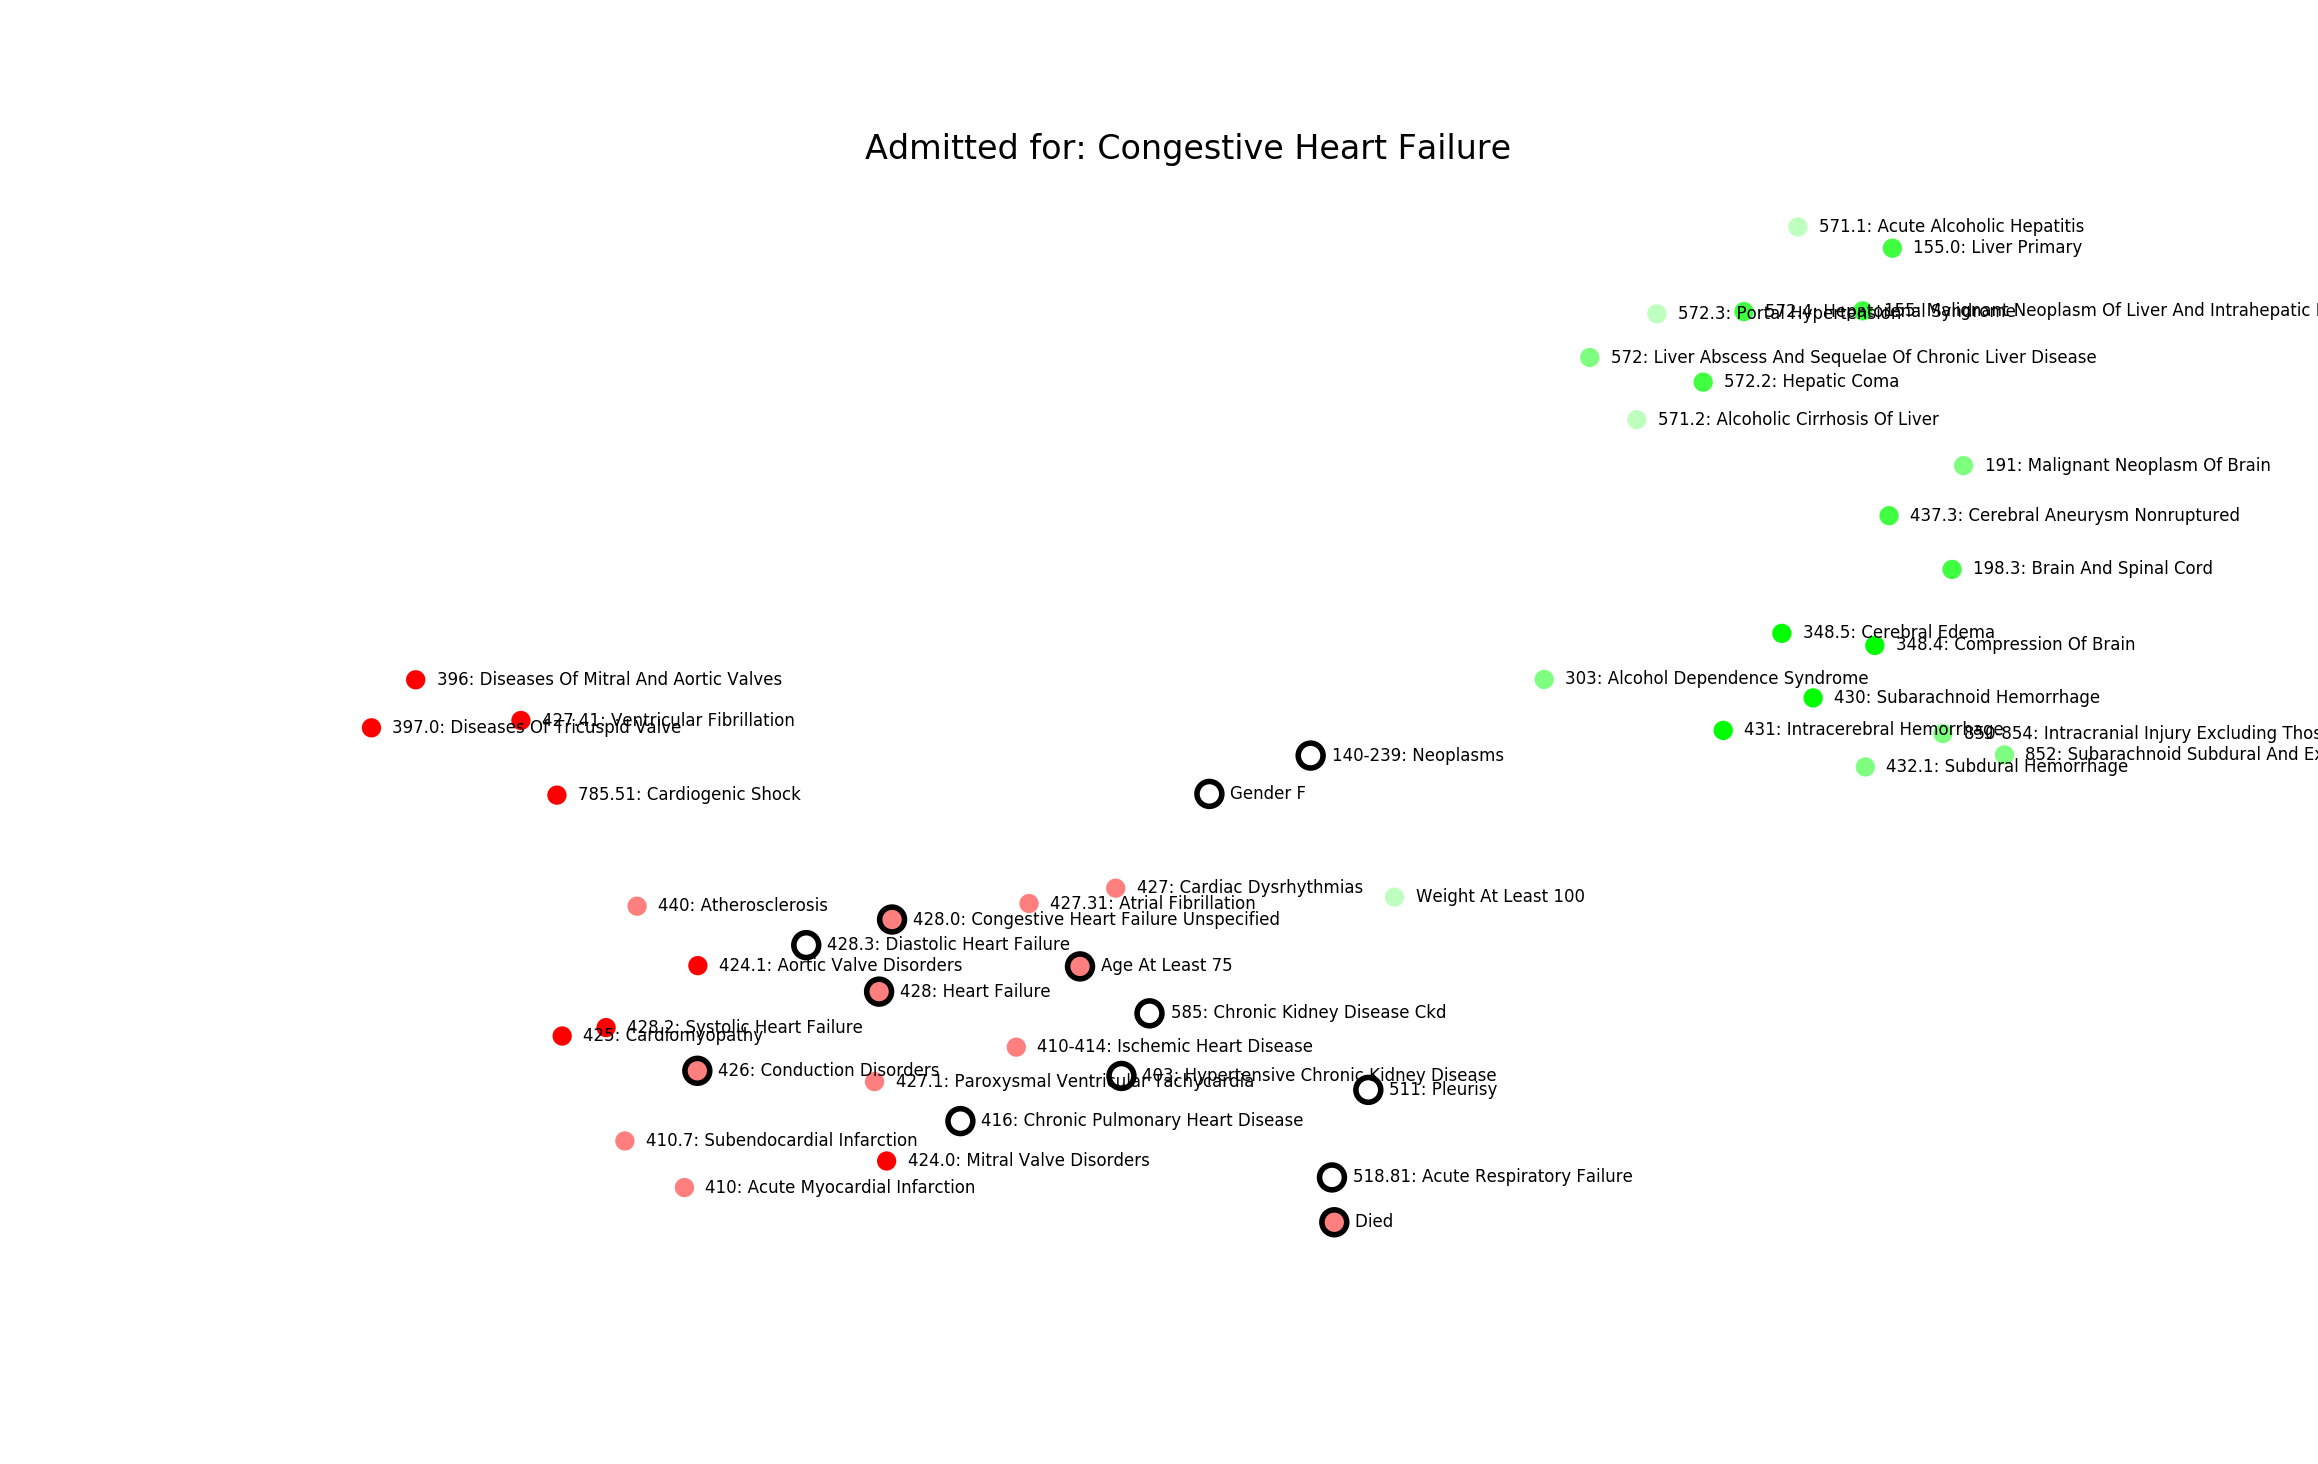
\includegraphics[width=\textwidth]{icu_map_chf}
    \caption{Semantic Inference Congestive Heart Failure}
    \vspace{12px}
    This patient was admitted for "Congestive Heart Failure".  The neural net predicted that they had low risk of liver and brain conditions (colored green).  It predicted high risk of heart conditions (colored red).  The patients was eventually diagnosed of conditions affecting the heart, and died (circled in black).
    \label{fig:icu_map_chf}
    \end{figure}
    
    \begin{figure}
    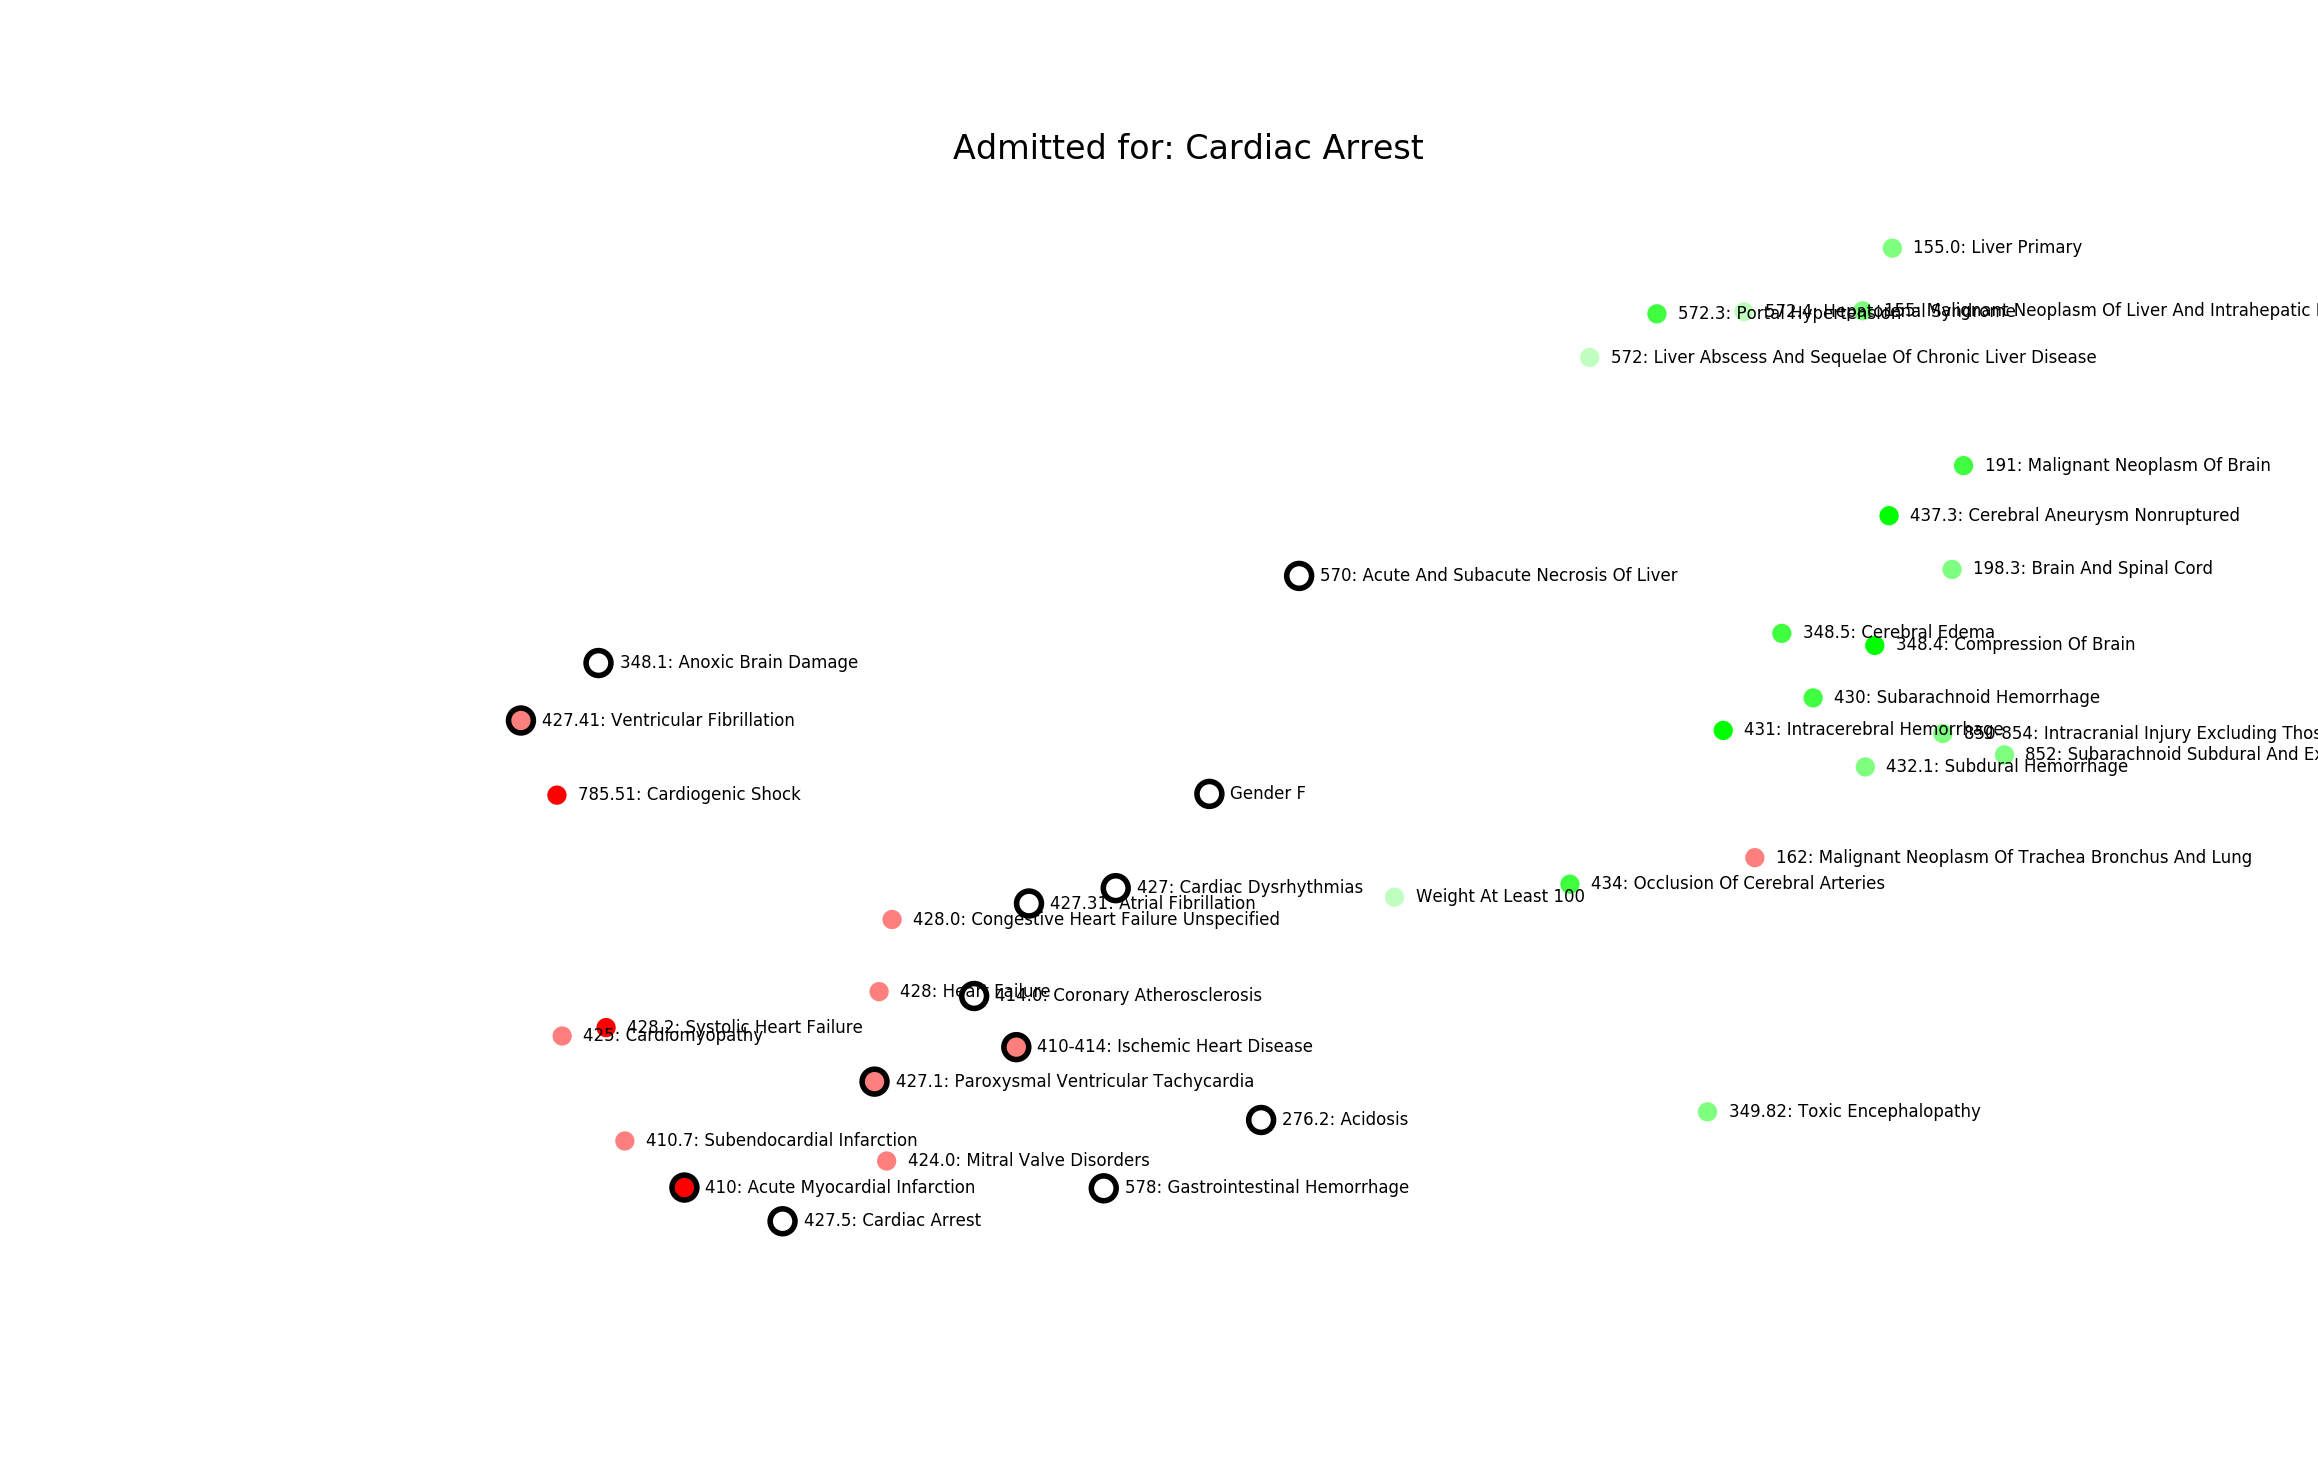
\includegraphics[width=\textwidth]{icu_map_cardarr}
    \caption{Semantic Inference Cardiac Arrest}
    \vspace{12px}
    This patient was admitted for "Cardiac Arrest".  The neural net predicted that they had low risk of liver and brain conditions (colored green).  It predicted high risk of heart conditions (colored red).  The patients was eventually diagnosed of conditions affecting the heart among other things (circled in black).
    \label{fig:icu_map_cardarr}
    \end{figure}
    
    \begin{figure}
    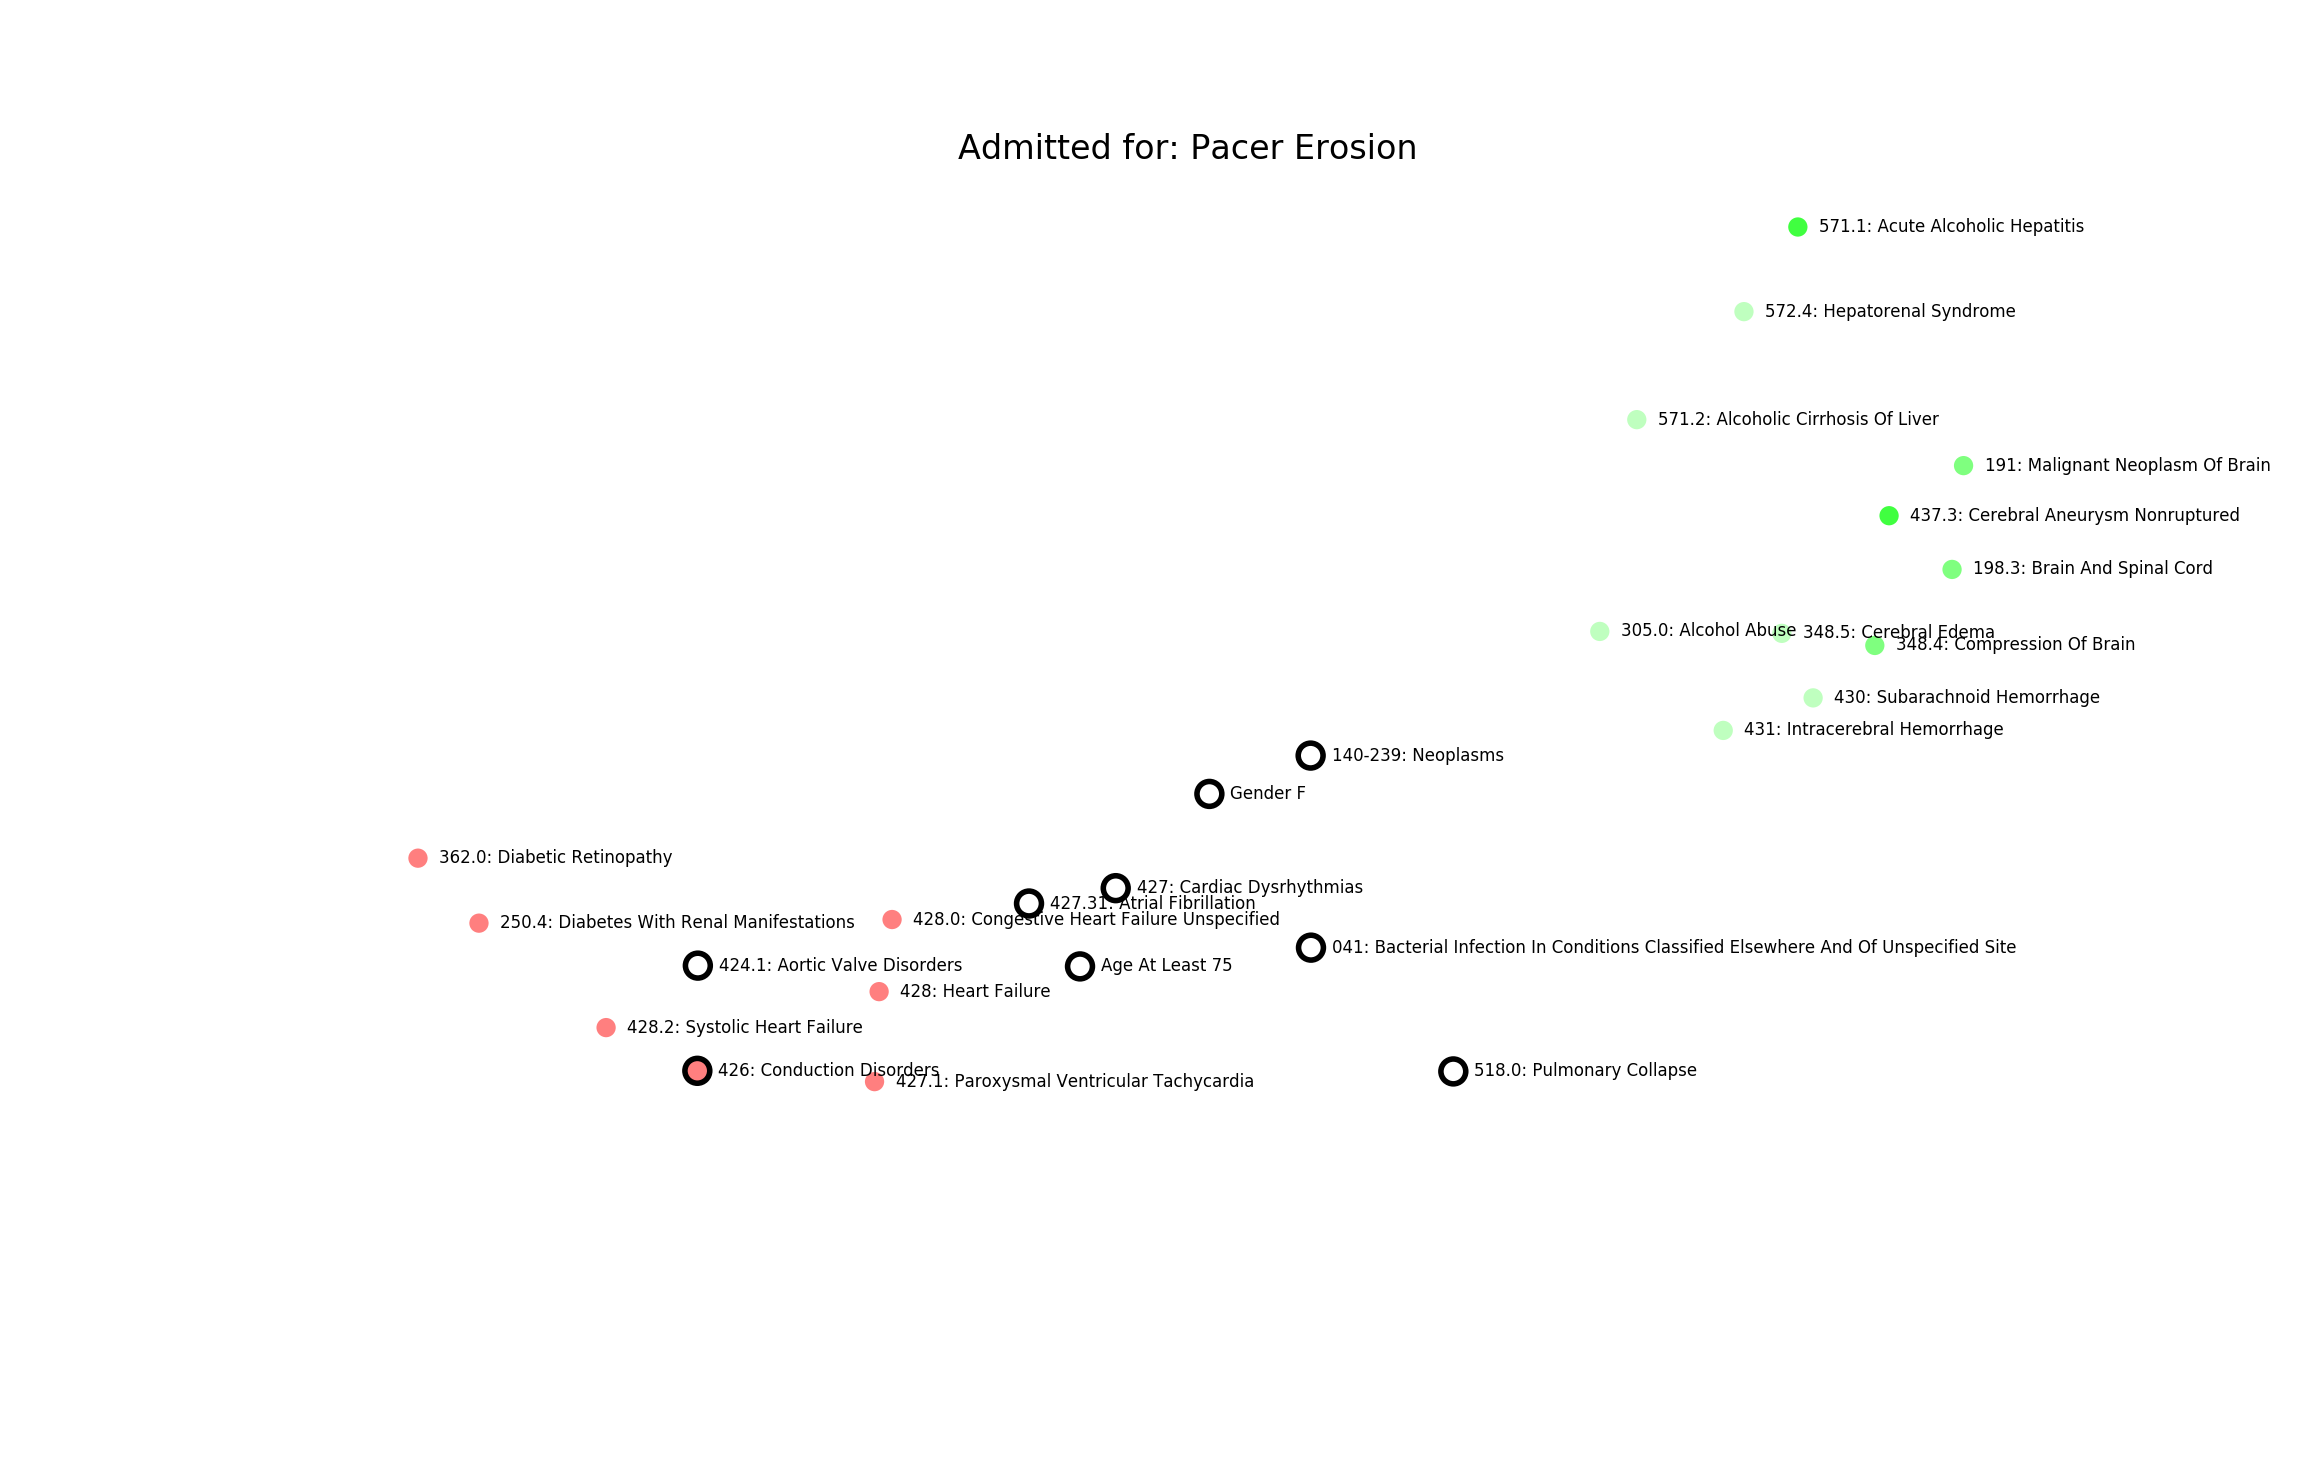
\includegraphics[width=\textwidth]{icu_map_pacer}
    \caption{Semantic Inference Pacer Erosion}
    \vspace{12px}
    This patient was admitted for "Pacer Erosion".  The neural net predicted that they had low risk of liver and brain conditions (colored green).  It predicted high risk of heart conditions (colored red).  The patients was eventually diagnosed of conditions affecting the heart (circled in black).
    \label{fig:icu_map_pacer}
    \end{figure}
    
    \begin{figure}
    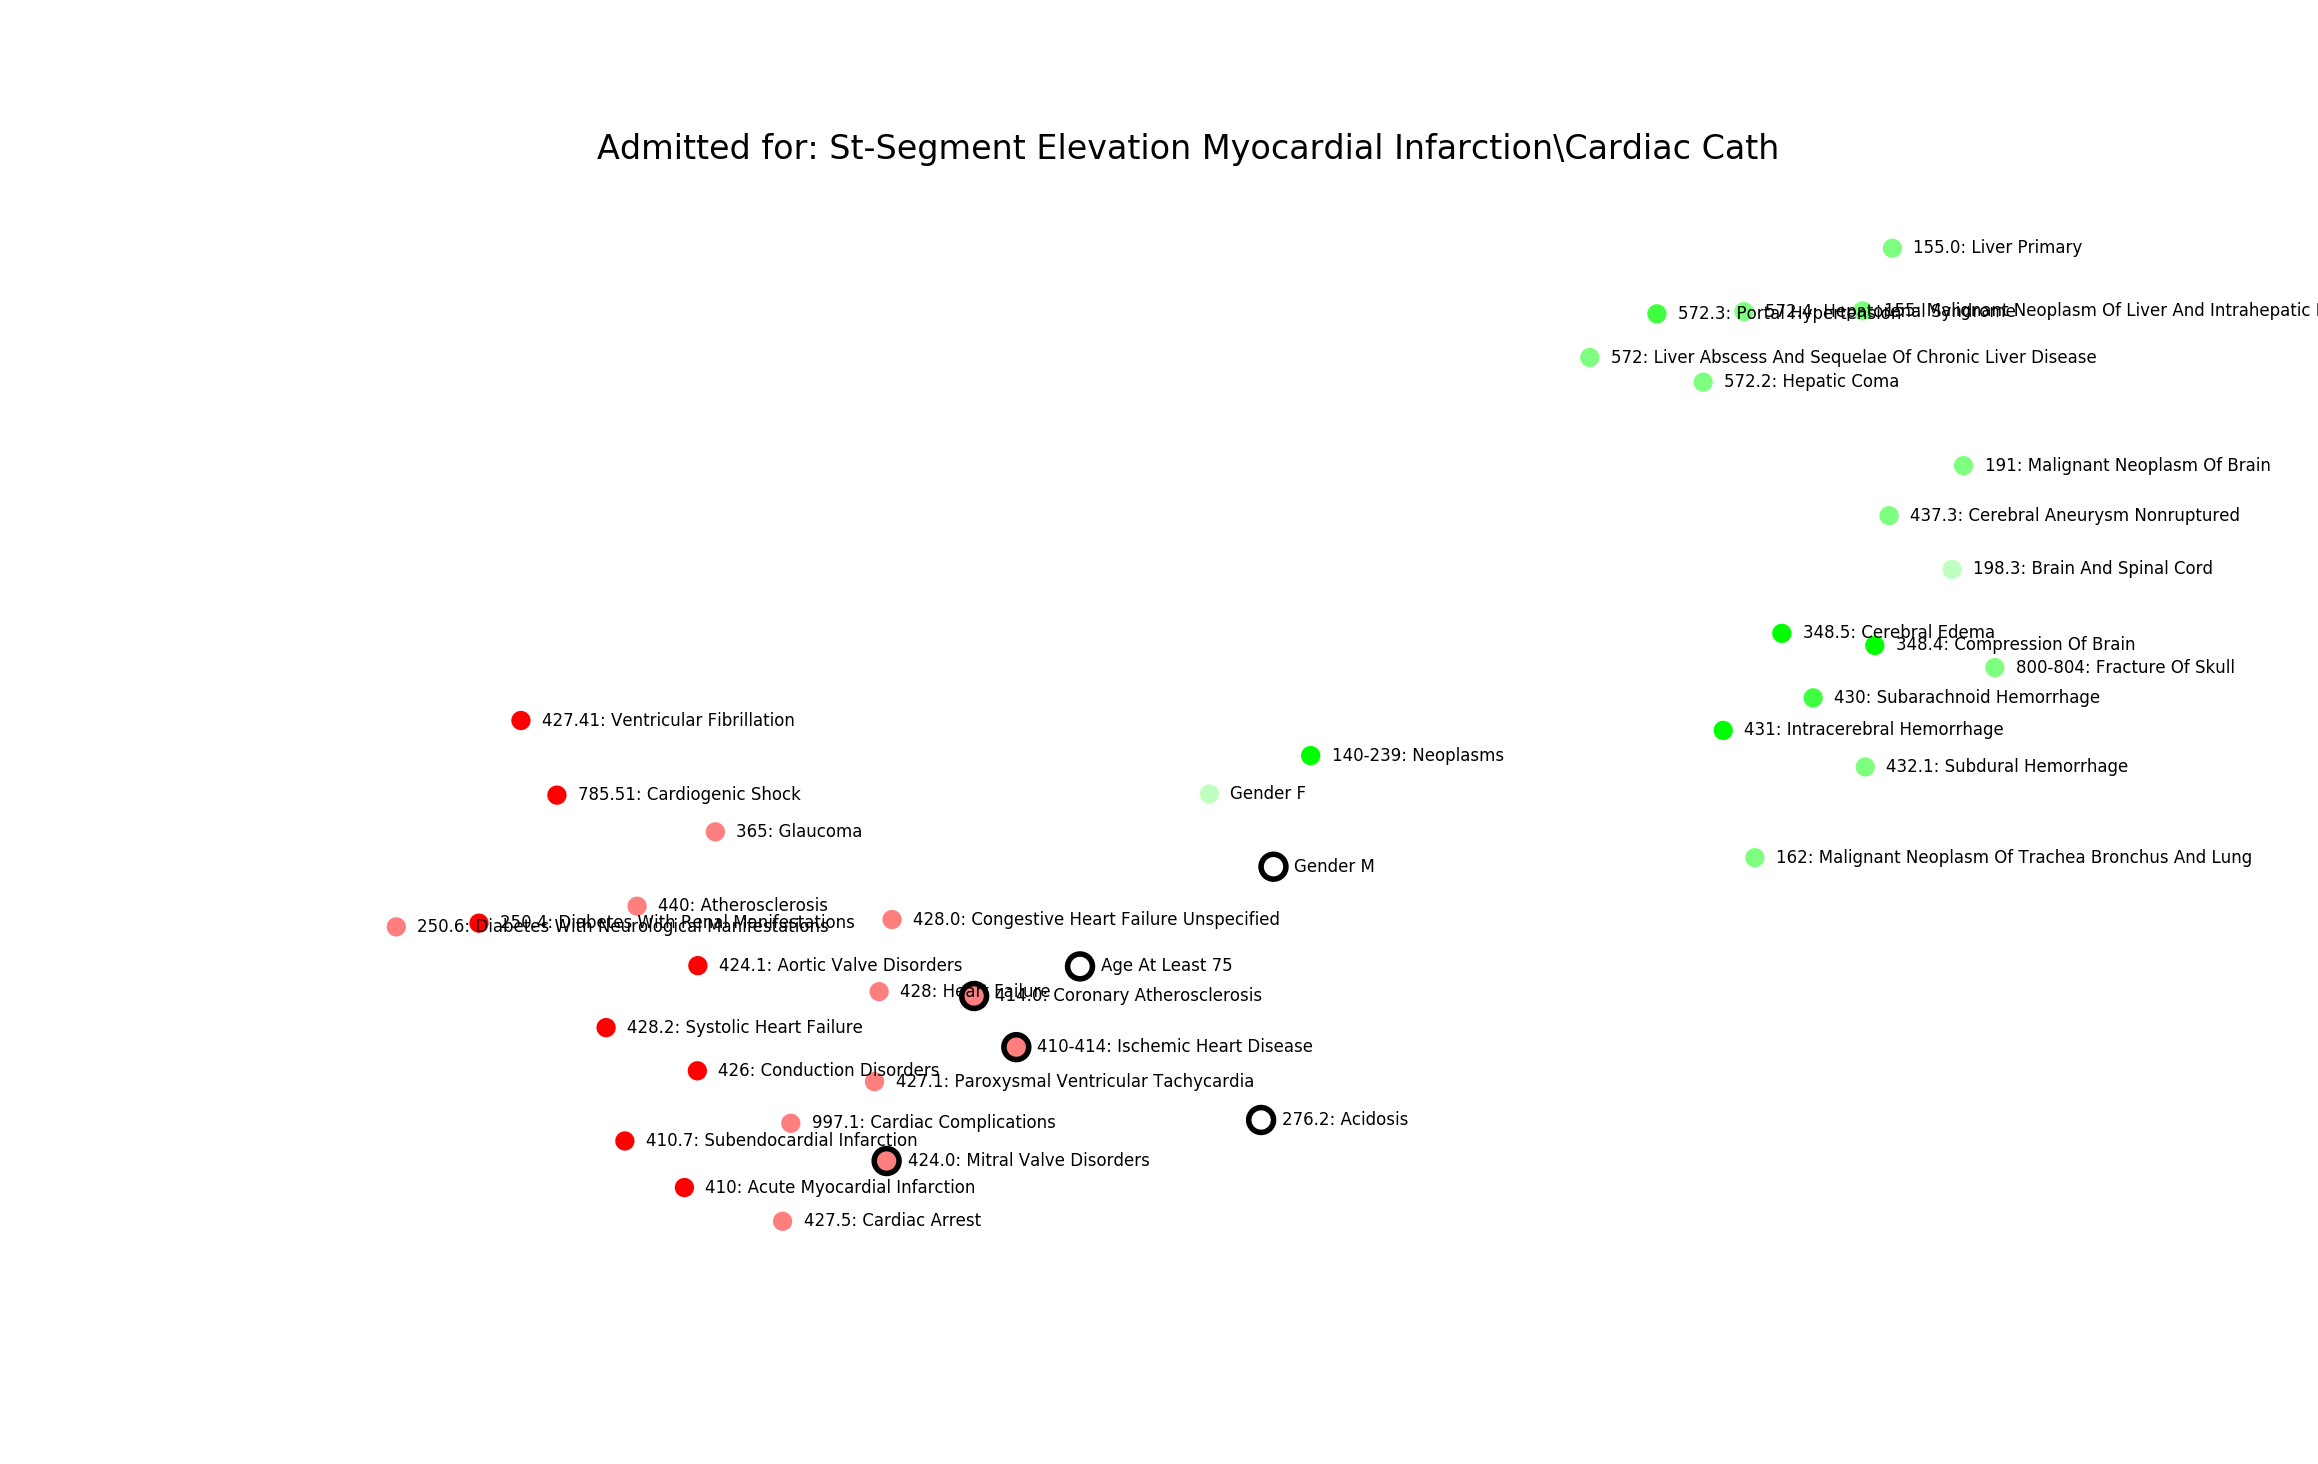
\includegraphics[width=\textwidth]{icu_map_stseg}
    \caption{Semantic Inference ST Elevation}
    \vspace{12px}
    This patient was admitted for "St-Segment Elevation Myocardial Infarction/Cardiac Cath".  The neural net predicted that they had low risk of liver and brain conditions (colored green).  It predicted high risk of heart conditions (colored red).  The patients was eventually diagnosed of conditions affecting the heart (circled in black).
    \label{fig:icu_map_stseg}
    \end{figure}
    
    \begin{figure}
    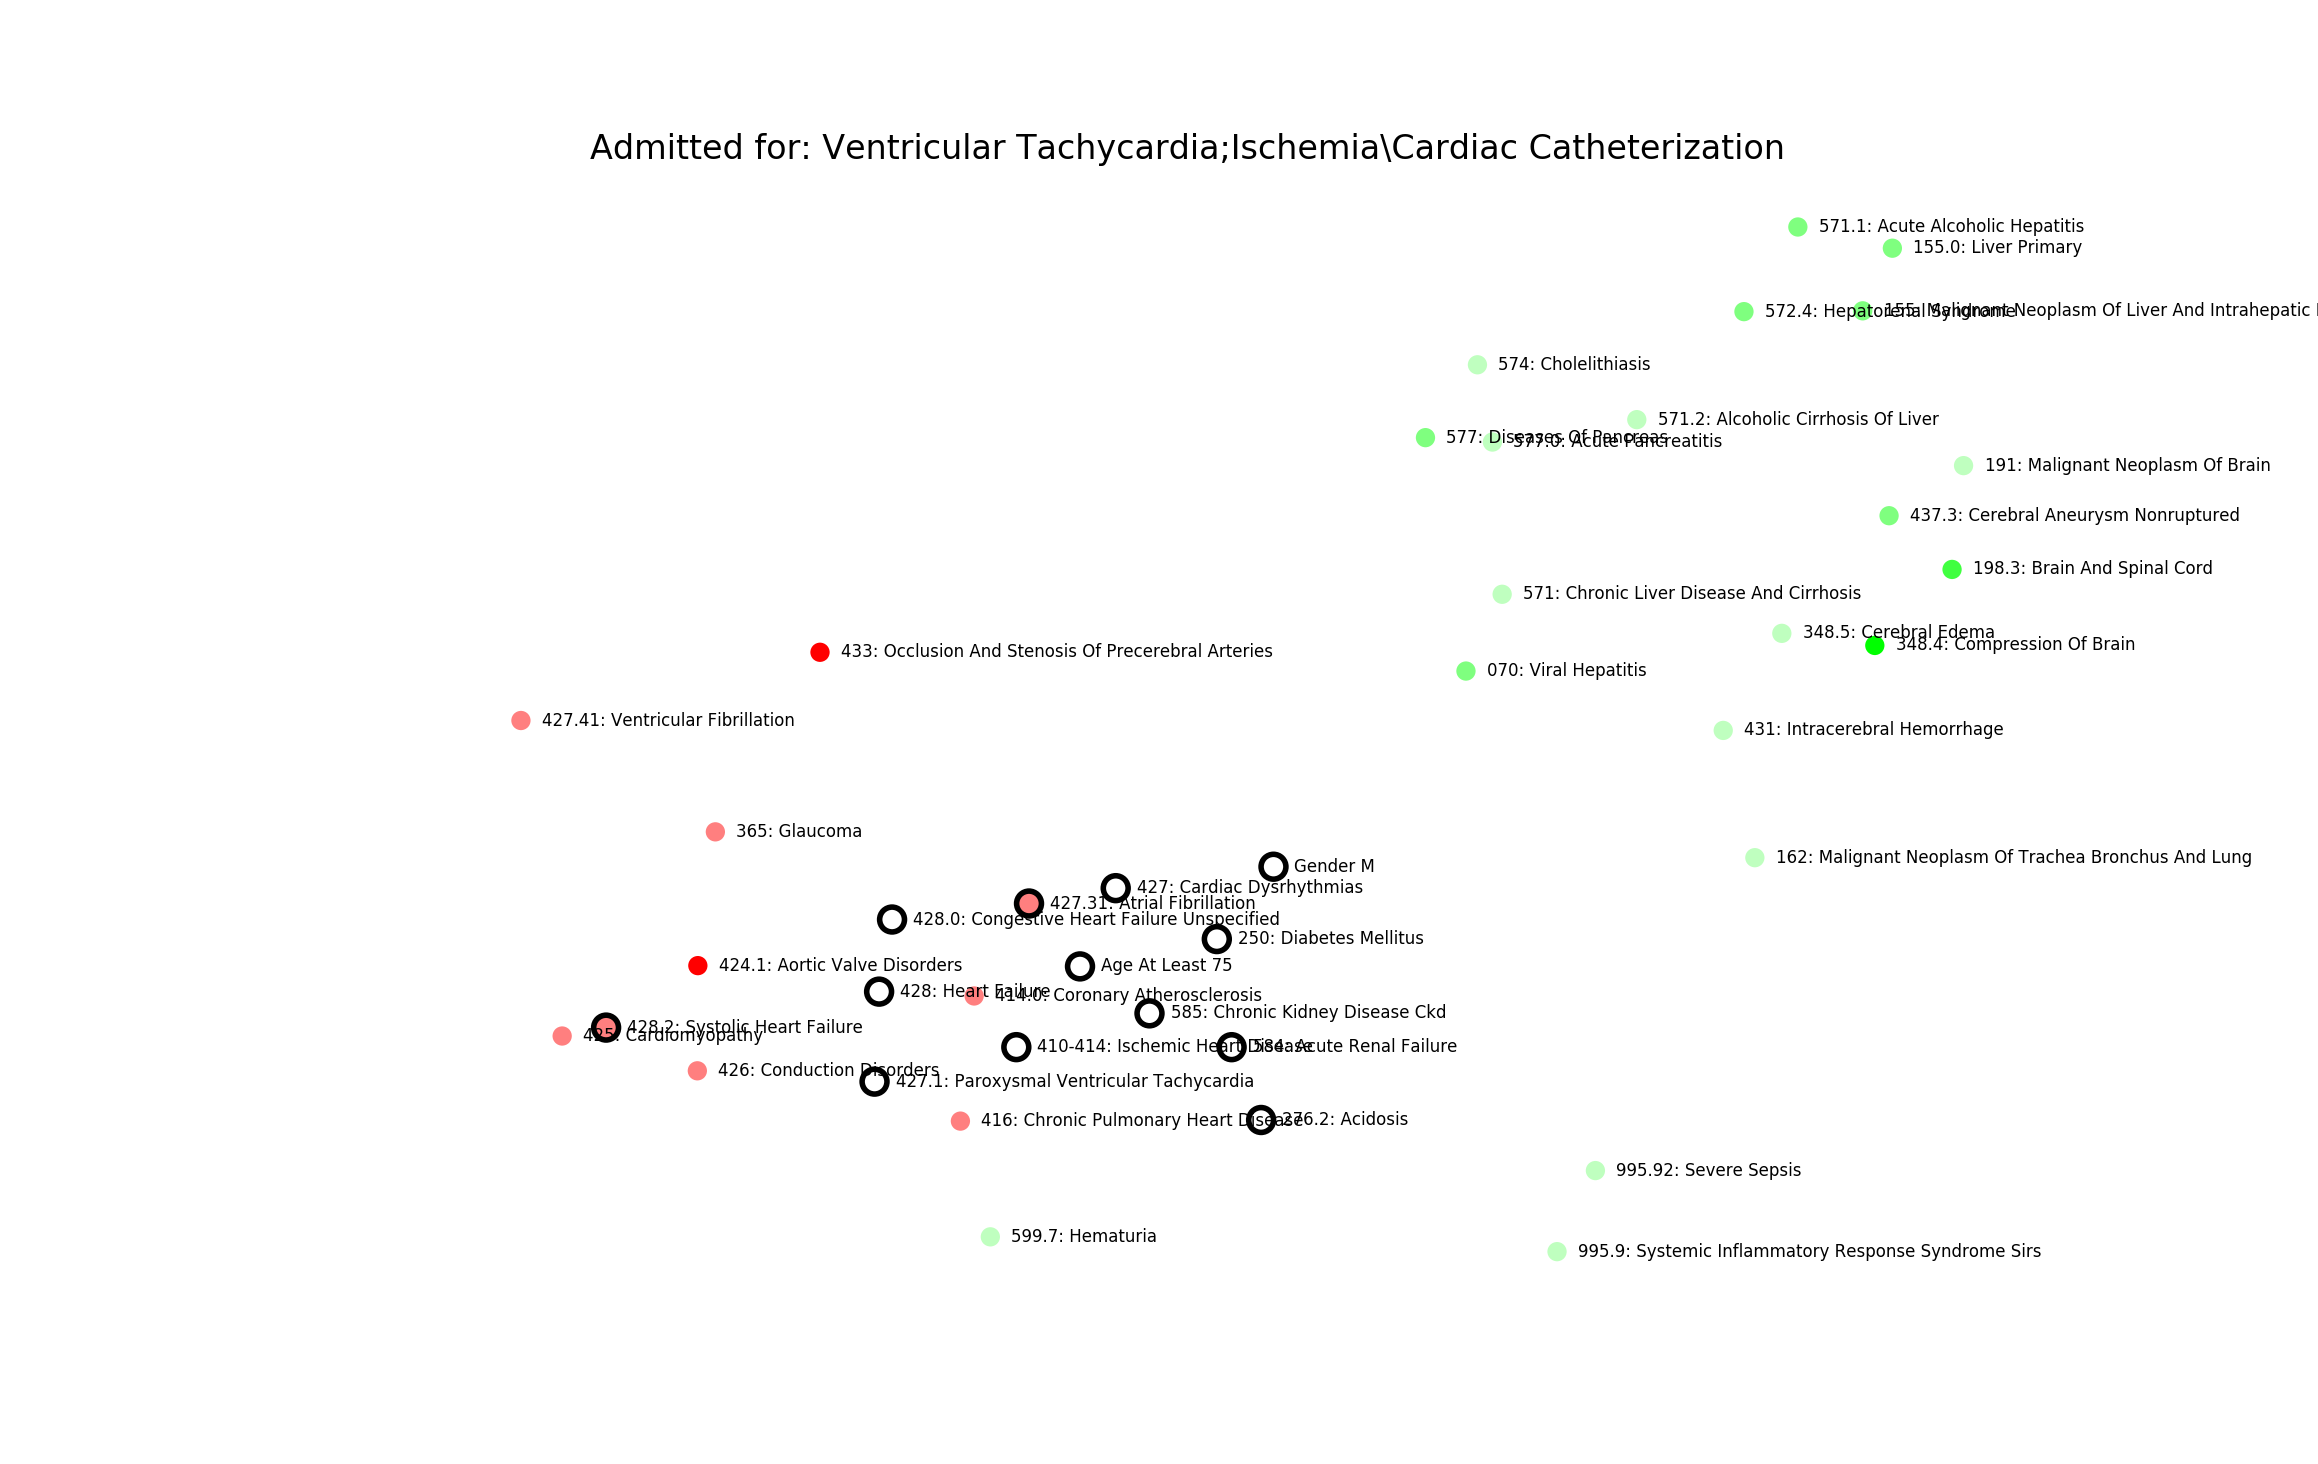
\includegraphics[width=\textwidth]{icu_map_ventach}
    \caption{Semantic Inference Ventricular Tachycardia}
    \vspace{12px}
    This patient was admitted for ventricular tachycardia.  The neural net predicted that they had low risk of liver and brain conditions (colored green).  It predicted high risk of heart conditions (colored red).  The patients was eventually diagnosed of conditions affecting the heart (circled in black).
    \label{fig:icu_map_ventach}
    \end{figure}
    
    \begin{figure}
    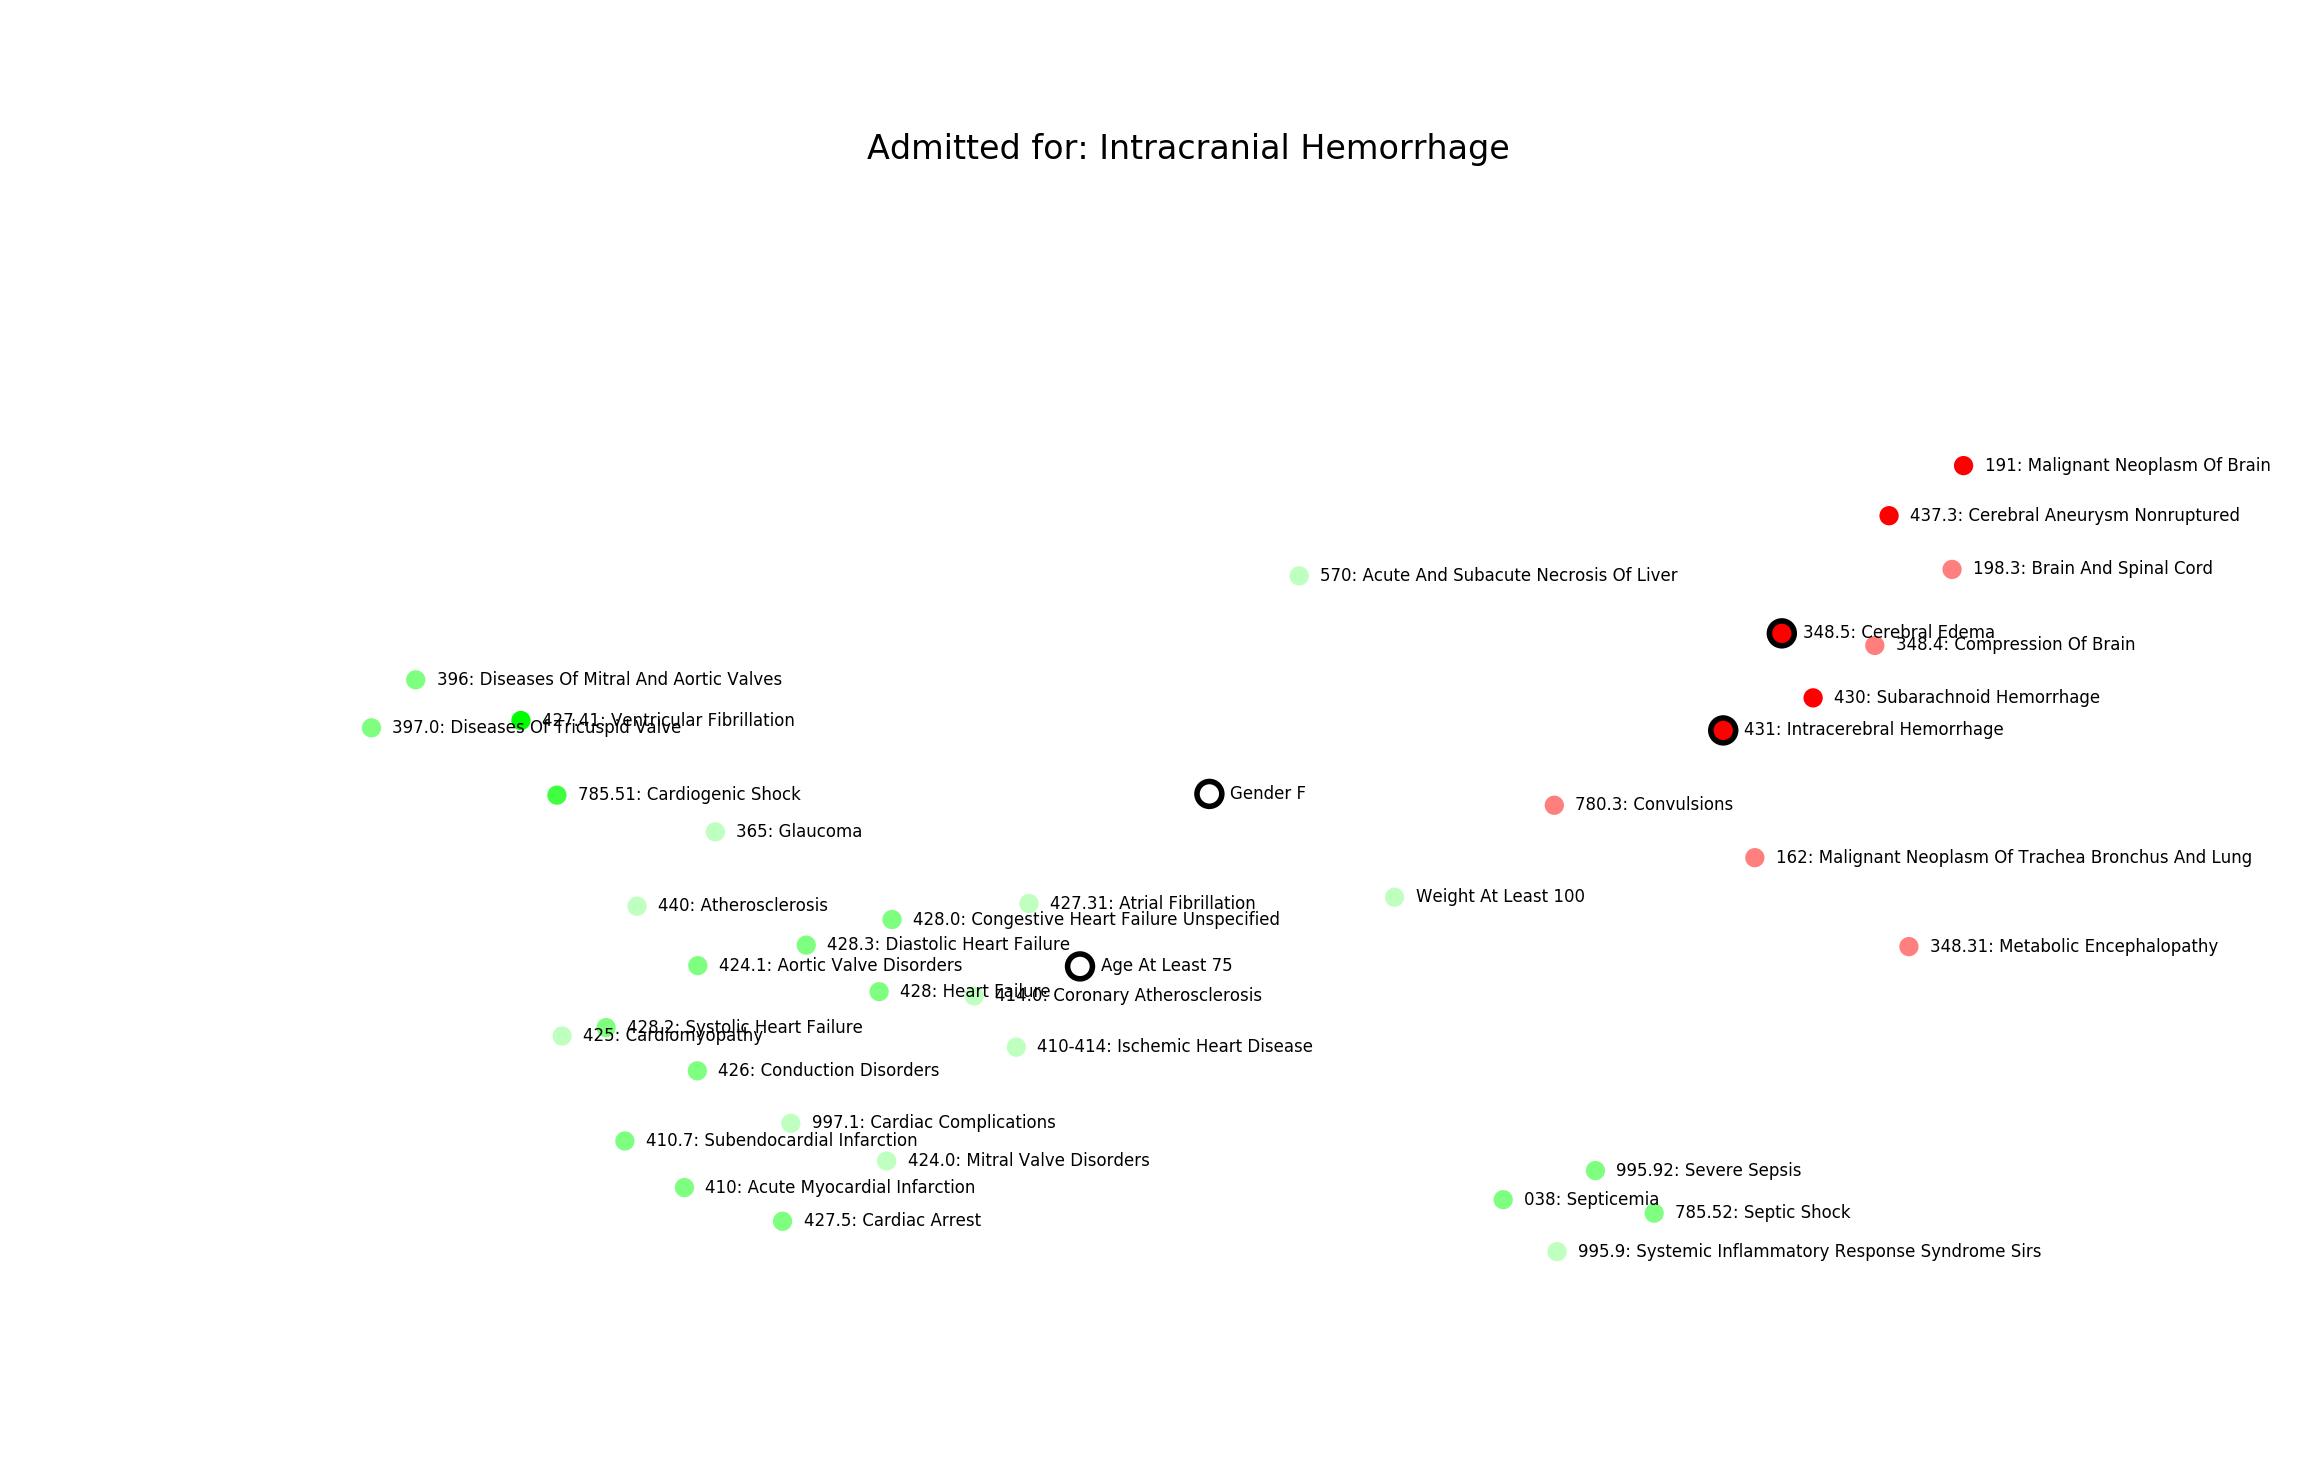
\includegraphics[width=\textwidth]{icu_map_brain}
    \caption{Semantic Inference Intracranial Hemorrhage}
    \vspace{12px}
    This patient was admitted for "Intracranial Hemorrhage".  The neural net predicted that they had low risk of heart conditions and septic conditions (colored green).  It predicted high risk of brain conditions (colored red).  The patients was eventually diagnosed with cerebral edema and intracerebral hemorrhage (circled in black).
    \label{fig:icu_map_brain}
    \end{figure}
    
    \begin{figure}
    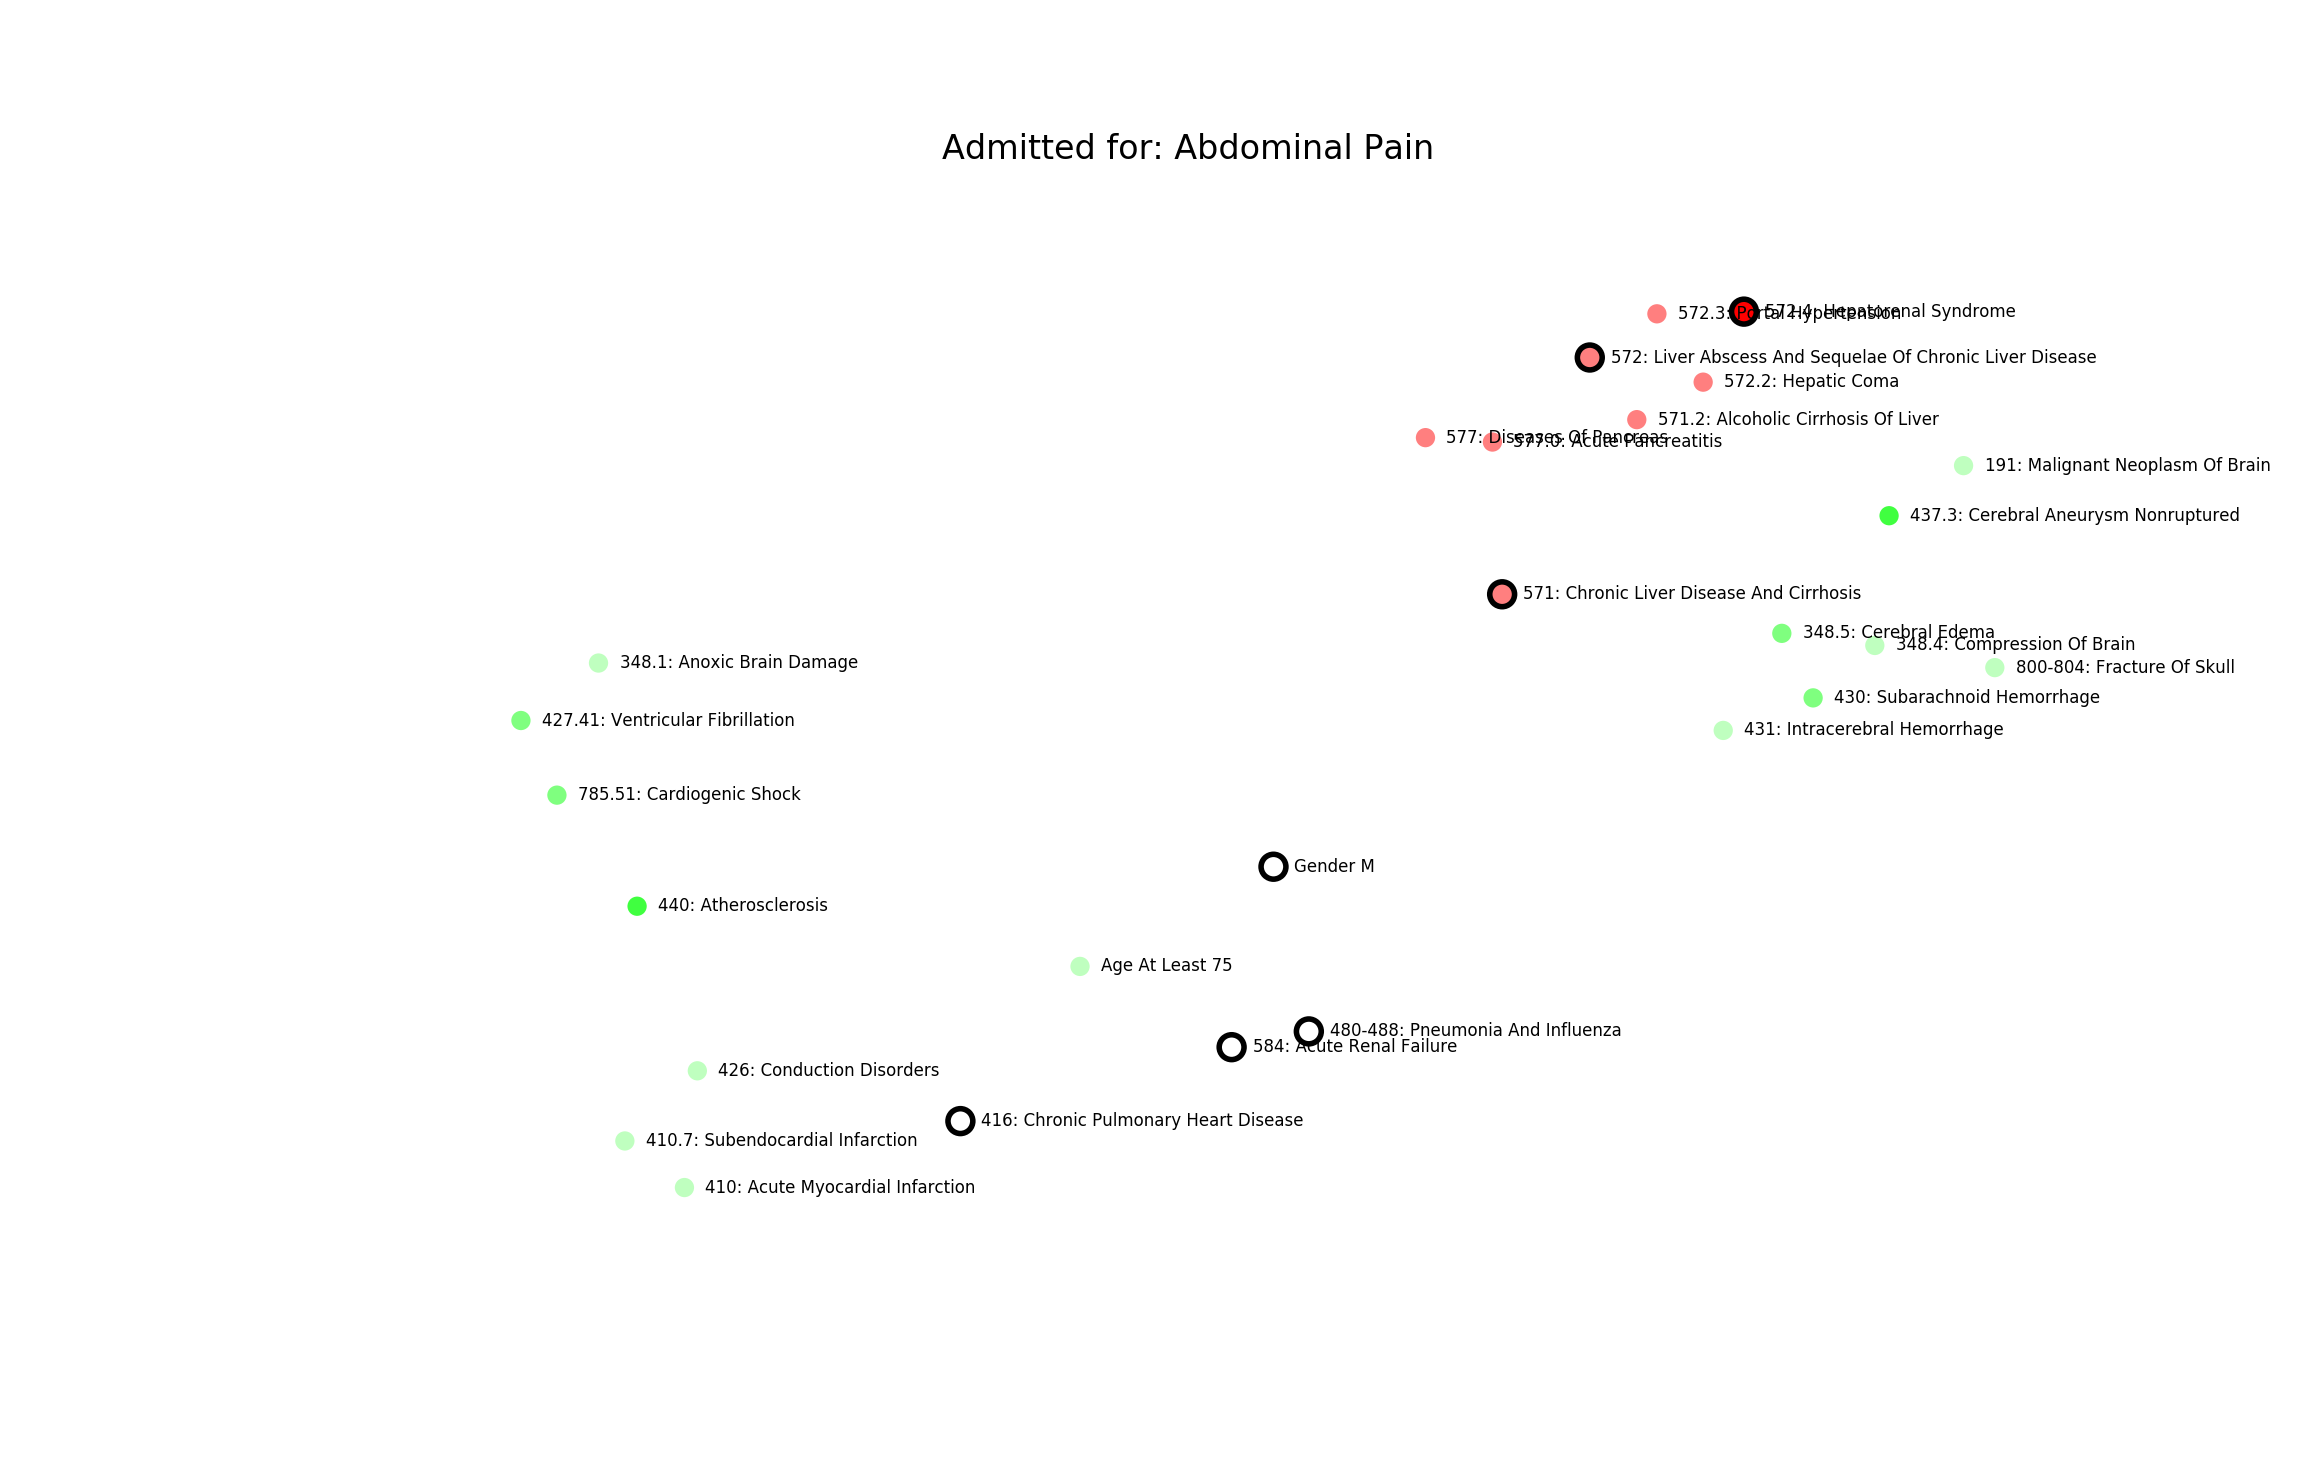
\includegraphics[width=\textwidth]{icu_map_liver}
    \caption{Semantic Inference Abdominal Pain}
    \vspace{12px}
    This patient was admitted for "Abdominal Pain".  The neural net predicted that they had low risk of brain and heart conditions (colored green).  It predicted high risk of liver conditions (colored red).  The patients was eventually diagnosed with chronic liver cirrhosis and a liver abscess among other things (circled in black).
    \label{fig:icu_map_liver}
    \end{figure}
}

\chapter{Critical Care}

\section{Introduction}
Wearable devices are becoming more common.  Over 100 million people wear an Apple Watch \cite{cybart_2021}.  This device is capable of measuring both a photoplethysmogram (PPG) and an electrocardiogram (ECG).  It has been FDA approved to detect atrial fibrillation, an irregular beating of the heart \cite{perez2019large}.  Maybe these devices can used to detect other conditions as well.  While smartwatch ECG and PPG data is not yet openly available in large quantities, there are large amounts of data available to researchers for patients in hospital intensive care units (ICU) \cite{johnson2016mimic}.  That is, the waveforms that smartwatches measure are also measured in ICUs, and ICU data is abundantly available for researchers.

The distribution of patients in an ICU is somewhat different from the distribution of smartwatch users.  Can detecting conditions with ICU data make progress toward detecting conditions in smartwatch users?  As demonstrated \cite{kuprel2017dermatologist}, a network trained to recognize everyday objects like cats and dogs can be adapted to detect various skin conditions.  Images of everyday objects are significantly more abundant, and more easily labeled, than images of skin conditions.  Waveforms and diagnoses collected from sick patients in the ICU are significantly more abundant than waveforms and diagnoses collected from smartwatches.  Progress can be made toward detecting medical conditions with smartwatches by first training on an abundant data source with associated diagnosis labels.  

The specific problem of detecting conditions in ICU patients is itself important.  Admission to the ICU is associated with risk of acute mortality given critical illness for those patients, which can include shock and end organ damage. During this period, patients are closely monitored in the intensive care setting with both invasive and noninvasive sensor data and frequent lab monitoring in order to effectively determine and prevent complications of critical illness.  Physicians often use risk scores designed to identify and predict patients’ risk of conditions such as shock: general physiologic scoring like shock index, or more specifically septic shock (qSOFA score) \cite{seymour2016assessment} or cardiogenic shock, completing Fick’s formula for cardiac index, cardiac output, and stroke volume \cite{fick1870ueber}.  Can deep learning can be used to learn risk analyses from data?

The approach taken is to solve the specific problem of detecting medical conditions in ICU patients with known diagnoses.  This step is important for solving the broader problem of detecting medical conditions with a smartwatch, which itself is important for solving the even broader problem of detecting life threatening medical conditions early with ubiquitous sensors.

\section{Methods}

\subsection{Dataset}

A large hospital-scale dataset collected by MIT researchers in a Harvard teaching hospital, called MIMIC \cite{johnson2016mimic}, contains raw data collected from 53,423 distinct hospital admissions.  Only a subset of this enormous dataset was used.  In particular, the waveforms and diagnoses were used.  Diagnoses are coded for insurance billing purposes in a taxonomy called the International Classification of Diseases (ICD).  This taxonomy comprises all known medical conditions. See Figure \ref{fig:icu_icd_mi} for an example of how the ICD code for "Acute myocardial infarction" is categorized.  Each patient is diagnosed with a set of conditions per hospital admission.

For each hospital admission a set of waveforms are recorded, and each for different lengths of time.  Many waveforms are corrupt or invalid.  Many invalid measurements correspond to times when poor contact is made with the sensor.  In addition, the waveforms are misaligned by up to 500ms.  Waveforms were sampled at 125Hz.  Up to 15 different waveforms were measured per patient.  These waveforms include:

\begin{itemize}
    \item PLETH: Photoplethysmogram
    \item RESP: Respiration
    \item ABP: Arterial Blood Pressure
    \item CVP: Central Venous Pressure
    \item ICP: Intracranial Pressure
    \item PAP: Pulmonary Arterial Pressure
    \item I, II, III, V, AVR, MCL: Electrocardiogram leads
\end{itemize}

\subsection{Preprocessing}

Much care was taken to transform the hospital-scale raw data dump into a form that a neural net could be trained with.  First the waveform records had to be matched to the chart information.  This was done using a patient identifier and timestamps.  Some of the waveforms were unable to be matched to a chart.  Second, not all patients had the same waveforms collected, and there was even variability within a patient of which waveforms were recorded. If a patient did not have a particular waveform measured, it is replaced with a vector of 0s.  For inference, only patients with a predefined set of waveforms measured were used.

\figIcuIcdMi
\figIcuExampleWaveforms

Consider a cleaned dataset
\begin{gather}
    \mathcal{D} = \{
        (x_{ij}, y_i),
        \text{ for } i \in \{ 1, \dots, n \},
        \text{ for } j \in \{ 1, \dots, m_i \}
    \} \\
    x_{ij} \in \mathcal{X} = \mathbb{R}^{T \times k} \\
    y_i \in \mathcal{Y} = \{0, 1\}^d
\end{gather}

where

\begin{itemize}
    \item $n > 10,000$ is the number of patients in the cleaned dataset
    \item $m_i$ is the number of examples from patient $i$, since each patient is in the hospital for a different length of time, and possibly more than one admission
    \item $x_{ij}$ represents $k = 15$ waveforms with $T = 2048$ samples each, or about 16 seconds given that they are recorded at 125 Hz.
    \item $y_i$ represents the $d = 90$ diagnoses for patient $i$.  If patient $i$ has ever once been diagnosed with diagnosis $j$ in any hospital admission on record, then $y_{ij} = 1$.  Otherwise, $y_{ij} = 0$
\end{itemize}

Let the net be described by a function $f$ that takes as input $x$ an example comprised of $k=15$ different waveforms each with $T=2048$ samples.  The net is also given parameters $\theta \in \Theta = \mathbb{R}^s$.  The net used contained $s = 6,721,114$ parameters.  The net outputs a vector of binary outcome probabilities $p$, one probability for each of the $d=90$ ICD codes.

\begin{gather}
    f: \mathcal{X} \times \Theta \mapsto \mathcal{P} = [0, 1]^d \\
    p = f(x, \theta)
\end{gather}

When the net makes a prediction, it is penalized by a loss function $\ell$.  The loss function takes as input the vector of binary-outcome probabilities $p$ that the net predicted, along with the vector of actual ICD code diagnoses $y$.  The loss is computed the binary cross entropies of these binary outcome probabilities and certain label probabilities (i.e. 0\% or 100\%), and then averaged over all ICD codes.

\begin{gather}
    \ell: \mathcal{P} \times \mathcal{Y} \mapsto \mathbb{R} \\
    \ell(p, y) = -\frac{1}{d} \sum_{j=1}^d 
        y_j * \log p_j + (1 - y_j) * \log(1 - p_j)
\end{gather}

The net is trained with batches of examples of size $b = 32$.  The batch loss $L$ is simply the sum of individual losses $\ell$.

\begin{gather}
    L : \mathcal{X}^b \times \mathcal{Y}^b 
        \times \Theta \mapsto \mathbb{R} \\
    X \in \mathcal{X}^b, Y \in \mathcal{Y}^b \\
    \begin{aligned}
        L(X, Y, \theta) 
            &= \sum_{i=1}^b \ell(f(x_i, \theta), y_i) \\
            &= \sum_{i=1}^b \ell(p_i, y_i) \\
            &= -\frac{1}{d} \sum_{i=1}^b \sum_{j=1}^d 
                y_{ij} * \log p_{ij} + (1 - y_{ij}) * \log(1 - p_{ij})
    \end{aligned}
\end{gather}

The parameters $\theta$ are computed with stochastic gradient descent.  The batch loss $L$ is differentiable with respect to the $k$th parameter of $\theta$.

\begin{align}
    \frac{\partial L}{\partial \theta_k} 
        &= \sum_{i=1}^b \sum_{j=1}^d 
            \frac{\partial \ell}{\partial p_{ij}}  
            \frac{\partial p_{ij}}{\partial \theta_k} \\
        &= \frac{1}{d} \sum_{i=1}^b \sum_{j=1}^d
            \left(
                \frac{1 - y_{ij}}{1 - p_{ij}} - \frac{y_{ij}}{p_{ij}}
            \right)
            \frac{\partial p_{ij}}{\partial \theta_k}
\end{align}

To complete this batch loss derivative, the net $f$ must take a form that is differentiable with respect to $\theta$.

% In matrix-vector form we have

% \begin{gather}
%     \frac{\partial L}{\partial \theta} = 
%         \sum_{i=1}^b 
%         \frac{\partial p_i^\intercal}{\partial \theta} 
%         \frac{\partial \ell}{\partial p_i}
% \end{gather}

\subsection{Model Architecture}

To take advantage of the stationary process nature of the waveforms, a 1D ConvNet was used.  If the waveforms were properly aligned, it would make sense to have convolution kernels span all the waveforms at once and convolve along the time dimension.  The waveforms, however, are not properly aligned.  They are misaligned by up to 500 ms, or about 64 samples.  This is on the order of the entire size of a convolution kernel.  In fact, the largest convolution kernels in the entire net were only 16 samples long.  To deal with the misalignment, the first 4 layers of the net convolve along the waveforms independently.  After 4 layers, each activation has a larger receptive field.  Dilated convolutions were used to help with this.  Stacked dilated convolutions enable networks to have very large receptive fields with just a few layers, while preserving the input resolution throughout the network \cite{oord2016wavenet}.  

To understand dilated convolutions, consider a simple example in 1 dimension with a kernel $w \in \mathbb{R}^3$ and dilation factor of 2.

\begin{gather}
    z_i^{(\ell + 1)} = 
        w_0 * z_{i - 2}^{(\ell)} +
        w_1 * z_{i}^{(\ell)} +
        w_2 * z_{i + 2}^{(\ell)}
\end{gather}

Residual layers are used to train a deep network and avoid vanishing gradients \cite{he2016deep}.  These networks were originally developed for computer vision applications but can be used here as well.  A residual layer takes the form

\begin{gather}
    z^{(\ell + 1)} = f(z^{(\ell)}) + z^{(\ell)}
\end{gather}

These skip connections allow data and gradients to flow unimpeded by the layers, allowing for deeper networks to be trained more aggressively.

The first 4 layers of the net are 1D dilated independent convolutions with skip connections.  The remaining 8 layers are 1D dilated joint convolutions with skip connections.  Finally there is a dense layer at the end.  The biases of the final layer are initialized such that the network predicts the prior of that condition when first initialized.  That is, if the prevalence of some condition is $p$, then the bias is set to $\log p - \log(1 - p)$, the inverse sigmoid of $p$.  Predicting the prevalence minimizes the binary cross entropy if only the prevalence is known.

% \figIcuModelArch

\subsection{Partition}

Test patient indices $\mathcal{I}$ are partitioned randomly into 3 sets, ($\mathcal{I}_1$, $\mathcal{I}_2$, $\mathcal{I}_3$), to be used for 3-fold cross-validation.  Patient $i$ is a valid test patient if the set of signals recorded for their stay $\mathcal{S}_i$ contains all the required waveforms specified by the set $\mathcal{S}_{test}$

\begin{gather}
    \mathcal{S}_{test} = \{ \text{PLETH, ABP, RESP, II, V, AVR} \}
\end{gather}.

These waveforms were chosen because they were commonly measured in the dataset.  The 3-fold partition is then

\begin{align}
    \mathcal{I} 
        &= \{
            i \mid \mathcal{S}_{test} \subseteq \mathcal{S}_i 
            \text{ for } i \in \{1, \dots, n\} 
        \} \\
        &= \mathcal{I}_1 \cup \mathcal{I}_2 \cup \mathcal{I}_3 \text{ where }
            \mathcal{I}_1 \cap \mathcal{I}_2 = \emptyset, \mathcal{I}_1 \cap \mathcal{I}_3 = \emptyset
\end{align}

Each fold defines a training dataset $\mathcal{D}_{train}$ and a testing dataset $\mathcal{D}_{test}$.

A patient that does not have all of the required waveforms measured for testing is still used for training.  The missing waveforms are represented with 0s.

A validation set wasn't used because the net was simply trained until the training loss started to plateau.  In prior experiments, this was fairly consistent with when the validation loss started to increase, i.e. the net was overfitting.  An entire validation set to determine when to stop training was determined not to be a good use of precious data.  

The training and testing datasets are defined as

\begin{gather}
    \mathcal{D}_{test} = \{
        (x_{ij}, y_i),
        \text{ for } i \in \mathcal{I}_k,
        \text{ for } j \in \{ 1, \dots, m_i \}
    \} \\
    \mathcal{D}_{train} = \{
        (x_{ij}, y_i),
        \text{ for } i \in \{1, \dots, n\} - \mathcal{I}_k,
        \text{ for } j \in \{ 1, \dots, m_i \}
    \}
\end{gather}

When training and testing, each patient has equal importance.  Since each patient was in the hospital for different lengths of time, this is achieved by randomly sampling a patient, and then randomly sampling a segment from their hospital stay.

\begin{gather}
    i \sim \text{uniform}(\mathcal{I}) \\
    j \sim \text{uniform}(\{1, \dots, m_i\})
\end{gather}

The per-patient example count $m_i$ can then be replaced by a constant $m$, since each patient has the same number of random examples drawn.  That is

\begin{gather}
    \mathcal{D} = \{
        (x_{ij}, y_i),
        \text{ for } i \in \{ 1, \dots, n \},
        \text{ for } j \in \{ 1, \dots, m \}
    \}
\end{gather}

% See the appendix for a more detailed model architecture summary.

\section{Results}

After performing 3-fold cross validation, there is a prediction for every example in the test set.

\begin{gather}
    \mathcal{P} = \{
        p_{ij},
        \text{ for } i \in \mathcal{I},
        \text{ for } j \in \{ 1, \dots, m \}
    \}
\end{gather}

\subsection{Relative Risk}

Just before the final sigmoid, there is an unnormalized representation of the net output.  That is $p = \text{sigmoid}(z)$ where $z \in \mathbb{R}$ and $p \in [0, 1]$.

\begin{gather}
    \mathcal{Z} = \{
        z_{ij},
        \text{ for } i \in \mathcal{I},
        \text{ for } j \in \{ 1, \dots, m \}
    \}
\end{gather}

The empirical conditional distributions over $z$ given $y$ can be used to compute a posterior.  Let $Y_k = 1 \mid Z_k = z$ be the event that an unseen patient is diagnosed with ICD code $k$ given that the net output value $z_k$ for that code.  Information on the reverse situation is known.  That is, there is information on the probability of the net outputting a value $z_k$ given that the patient is or is not diagnosed.  The prevalences of these conditions in the hospital are also known.  Let $\pi_k$ be the prevalence of ICD code $k$ among hospital patients.  Applying Bayes Rule:

\begin{gather}
    P(Y_k = 1 \mid Z_k = z) = \frac
        {P(Z_k = z \mid Y_k = 1) \ \pi_k}
        {P(Z_k = z \mid Y_k = 0) (1 - \pi_k) + P(Z_k = z \mid Y_k = 1) \ \pi_k}
\end{gather}

To compute this distribution, one would first need to compute histograms of $z$ given $sick$ ($y=1$) and of $z$ given not $sick$ ($y=0$).  That is, bin possible values of $z$ and count how many times the net predicts a value within that range.  Finally normalize that histogram so that the total area is 1.  If the bins are too small, the number of occurrences in a particular bin has high variance, and the empirical distribution will be far from smooth.  If the bins are too large, the empirical distribution will be very coarse.  Is there a more direct way, to avoid binning and counting?  Yes, there is Kernel Bayes Rule \cite{fukumizu2013kernel}.  

Kernel Bayes Rule says that given a bunch of observations $(x_i, y_i)$ for $i = 1, \dots, n$, the posterior of $y$ given $x$ can be estimated as

\begin{gather}
    P(Y = y | X = x) = \frac
        {\sum_{i=1}^n K(x - x_i) \ K(y - y_i)}
        {\sum_{i=1}^n K(x - x_i)}
\end{gather}

Where $K: \mathbb{R} \mapsto \mathbb{R}$ is a positive definite kernel function.

Applying Kernel Bayes Rule, the posterior can be directly computed.

\begin{gather}
    P(Y_k = 1 \mid Z_k = z) = \frac
        {\sum_{i=1}^n y_{ik} \sum_{j=1}^m K(z - z_{ijk})}
        {\sum_{i=1}^n \sum_{j=1}^m K(z - z_{ijk})}
\end{gather}

A standard radial basis function (RBF) kernel was used with $\sigma = 0.8$.  See Figure \ref{fig:icu_cardio_prob} for conditional kernel densities of the net's prediction for the ICD code of cardiogenic shock, given whether the patient does or does not end up having a cardiogenic shock.

When computing this posterior, it is important to maintain the condition that no prediction should depend on its label.  This sounds pretty obvious but is easily neglected here.

To see why, consider the posterior calculation written out in its full glory:

\begin{gather}
    P(y_{ik} = 1 \mid z_{ijk} = z) = \frac
        {\sum_{i' \in \mathcal{I}} y_{i'k} \sum_{j'=1}^m K(z - z_{i'j'k})}
        {\sum_{i' \in \mathcal{I}} \sum_{j'=1}^m K(z - z_{i'j'k})}
\end{gather}

There are two issues here.  First the summation over $\mathcal{I}$ should instead be over $\mathcal{I} - i$, otherwise $y_{ik}$ is being used to predict $y_{ik}$.  Second, remember that $z_{ij} = f(x_{ij}, \theta)$, and $\theta$ is a function of $\mathcal{D}_{train}$, via gradient descent.  Therefore, any label contained in $\mathcal{D}_{train}$, and therefore, any prediction on an example in $\mathcal{D}_{train}$ cannot be used to compute the posterior.  It follows then compute a posterior without using the label in any way whatsoever, change the summation over all patients $\mathcal{I}$ to patients in the test set except for the test patient of interest $\mathcal{I}_{test} - i$.

\begin{gather}
    P(y_{ik} = 1 \mid z_{ijk} = z) = \frac
        {\sum_{i' \in \mathcal{I}_{test} - i} \sum_{j'=1}^m K(z - z_{i'j'k}) \ y_{i'k}}
        {\sum_{i' \in \mathcal{I}_{test} - i} \sum_{j'=1}^m K(z - z_{i'j'k})}
\end{gather}

The relative risk relative to the prevalence of that condition $r$ can be computed for every patient $i$ in the test set, for every example from their stay $j$, and for every ICD code $k$.

\begin{gather}
    \hat{r}_{ijk} = \frac
        {P(y_{ik} = 1 \mid z_{ijk} = z)}
        {\pi_k}
\end{gather}

We can bin the patients into relative risk category by powers of two, generating Figure \ref{fig:icu_relative_risk}.

Another useful thing to know at the patient level would be, how much more or less at risk am I than everyone else?  In medicine this metric is referred to as relative risk.  In other contexts it is referred to as risk ratio or Bayes factor.  In medicine, relative risk is usually used to compare “exposed” and “unexposed” groups.  We can calculate relative risk as the probability that a patient has a condition given the output of the ConvNet, divided by the prevalence of that condition.  To calculate the posterior we can use the kernel density estimates along with the prevalences.  It turns out there’s actually a direct way to calculate the posterior using kernel Bayes rule.  This avoids discretization and other unnecessary steps.

We can compute the relative risk for every patient in the test set.  Let’s group them by powers of 2.  A person in the 2x group is at twice or more the risk of having the condition but less than 4x, a person in the ½ group is less than half as likely to have the condition but more than 1/4x, and so on.  When we put every test patient into one of those risk groups for all of the ICD codes, we get the figure shown here.  Looking at cardiogenic shock, for example, we can put about half of the patients into a low risk group.

\figIcuRelativeRisk

How do we know these risk groups are valid?  For each risk group we can look at how often patients in that group were ultimately diagnosed with a condition compared to the prevalence.  We can compute that for each of the 90 diseases.  Here I show the mean and standard deviations of the actual risks associated with the target risk groups.  For higher risk groups, we would expect that the actual risk is higher than the target risk.  A patient placed in the 2x risk group had an estimated risk of anywhere from 2 to 4 times.  We do in fact see that the actual risk for high risk groups is higher than the estimated risk.  Similarly we see that the actual risk for low risk groups is lower than the estimated risk.

For risk group $g = (g_\text{min}, g_\text{max})$ and ICD code $k$, we have $\mathcal{F}_k$ as the set of examples $(i, j)$ that were flagged within that risk group.

\begin{gather}
    \mathcal{F}_k(g) = \{ (i, j) \mid g_{\text{min}} < r_{ijk} < g_{\text{max}} \} \\
    a_{k}(g) = \frac{1}{\pi_k} \left( 
        \frac{\sum_{(i, j) \in \mathcal{F}_k(g)} y_{ik}}{|\mathcal{F}_k(g)|}
    \right)
\end{gather}

In figure \ref{fig:icu_actual_risk} the means and standard deviations of actual risk for each risk group are plotted.  For group $g$ we have

\begin{gather}
    \mu(g) = \frac{1}{d} \sum_{k=1}^d a_k(g) \\
    \sigma^2(g) = \frac{1}{d} \sum_{k=1}^d (a_k(g) - \mu(g))^2
\end{gather}

\figIcuActualRisk

\subsection{Effective Sensitivity}

Assume there is a perfect, but expensive test.  There is also a cheap and ubiquitous test, but far from perfect.  Imagine for example, the situation of a smartwatch user.  The smartwatch can perform various measurements for little to no cost.  Can the cheap test be used to recommend patients get a more expensive test?  If the expensive test is used on 20\% of the patients sampled at random, it is expected to catch 20\% of the cases.  Then, the effective sensitivity of the perfect test is only 20\%, not 100\%, because it effectively reported false negative for the 80\% of patients not tested.  On the other hand, if patients are triaged according to the neural net output and the 20\% percent most at risk are tested, about 3 times the cases can be detected, see Figures \ref{fig:icu_cardio_prob} to \ref{fig:icu_myocard_sens}. It’s not hard to imagine a smartwatch app recommending people get MRI scans or other tests if they are at high risk according to a neural net.

We can calculate sensitivity as follows

\begin{align}
    \text{sensitivity}_k 
        &= \frac{TP_k}{TP_k + FN_k} \\
        &= \frac
            {\sum_{i \in \mathcal{I}} y_{ik} \hat{y}_{ik}}
            {\sum_{i \in \mathcal{I}} y_{ik}}
\end{align}

Imagine the test is perfect, that is $y_{ik} = \hat{y}_{ik}$ for all patients $i$ and ICD codes $k$.  But there is a limit on the number of patients that can be tested with this test, $\mathcal{J} \subset \mathcal{I}$, $|\mathcal{J}| < c$.  The untested patients are effectively predicted to not have the condition, that is $\hat{y}_{ik} = 0$ for $i \notin \mathcal{J}$.

\begin{align}
    \text{sensitivity}_k 
        &= \frac
            {\sum_{i \in \mathcal{I}} y_{ik} \hat{y}_{ik}}
            {\sum_{i \in \mathcal{I}} y_{ik}} \\
        &= \frac
            {\sum_{i \in \mathcal{J}} y_{ik}}
            {\sum_{i \in \mathcal{I}} y_{ik}} \\
        &\leq 1
\end{align}

The problem becomes to choose the best set of $c$ patients $\mathcal{J}$ to send to the perfect test.  If the chosen set of patients contains all patients who have that disease, the sensitivity will be 100\%. If the patients $\mathcal{J}$ are chosen randomly, the expected sensitivity is the percent of patients tested.

\begin{align}
    \mathbb{E}[\text{sensitivity}_k]
        &= \frac
            {\mathbb{E}[\sum_{i \in \mathcal{J}} y_{ik}]}
            {\sum_{i \in \mathcal{I}} y_{ik}} \\
        &= \frac{c * \pi_k}{n * \pi_k} = \frac{c}{n}
\end{align}

How much better can random than the neural net do?  See Figures \ref{fig:icu_cardio_prob} to \ref{fig:icu_myocard_sens}.

% \figIcuCardioProb
% \figIcuCardioSens
% \figIcuSystolicProb
% \figIcuSystolicSens
% \figIcuCerebralProb
% \figIcuCerbralSens
% \figIcuMyocardProb
% \figIcuMyocardSens

\subsection{Semantic Space Inference}

Just before the final sigmoid, we have another representation of the net output.  That is $p = \text{sigmoid}(z)$ where $z \in \mathbb{R}$ and $p \in [0, 1]$.  Create a large matrix of this output $Z \in \mathbb{R}^{n \times d}$ where $Z_{ik}$ represents the net output for ICD code $k$ for patient $i$.  The rows of this matrix are $d$ $n$-dimensional vectors representing each of the ICD codes.  These $n$-dimensional vectors can be embedded into 2 dimensions using TSNE \cite{van2008visualizing}.

\figIcuEmbeddingMethod

The result is shown in \ref{fig:icu_embedding_method}. Conditions are color coded by which part of the body they affect.  Red circles are conditions that affect the heart.  These conditions include cardiogenic shock, coronary atherosclerosis, atrial flutter, systolic heart failure, and myocardial infarction.  Green circles are conditions that affect the brain.  These conditions include cerebral edema, brain cancer, cerebral aneurysm, intracerebral hemorrhage.  It’s interesting that skull fracture found its way into this region.  Yellow circles are conditions that affect the liver.  These conditions include cirrhosis, hepatitis, and liver cancer.  It is interesting that alcohol abuse and alcohol dependence syndrome found their way into this region, and are also close to the brain conditions.  Blue circles are conditions that affect the lungs.  These conditions include pulmonary collapse, pneumonia, and acute respiratory failure.  It is remarkable that a highly articulate semantic space can be learned from simple waveforms.  Further it puts similar ICD codes together that may be far apart in the ICD taxonomy.  For example, in the center we have ICD code 785.52: Septic Shock, ICD code 995.92: Severe Sepsis, and ICD code 038: Septicemia.  The nearest common ancestor of these ICD codes in the taxonomy is the root of the entire taxonomy of all medical conditions that exist.  But the net learned that they were similar semantically based on the waveforms it was trained with.

\figIcuIcdMap

Now that we have this semantic space and relative risk computed for all the test patients, let's see what the net predicts on a patient by patient level.  Here the ICD codes are colored according to the risk level that patient has.  Actual diagnoses are circled in white.

% \figIcuMaps

\section{Conclusion}
Deep learning can improve learn to analyze risk of patients for various life threatening conditions given information from noninvasive measurements.  This can be directly applied to triage patients in the ICU.  It can be used to assess relative risk of a particular patient.  And if can be used to assess overall health condition within a semantic space of diseases.  The field of preventive care is far from perfect and the solution here is far from perfect.  But it is more useful than existing imperfect and non existing solutions.